\documentclass[final, 16pt]{beamer}
% poster
\usepackage[size=custom, width=95, height=120]{beamerposter}
% common stuff
\usepackage{graphicx}
\usepackage{hyperref}
\usepackage{booktabs}
\usepackage{amsmath}
\usepackage{caption}
\usepackage{subcaption}
\usepackage{array}
\usepackage{xparse}
\usepackage{wrapfig}
\usepackage{xspace}
% necessary acronyms
\def\ie{\textit{i.e.}\xspace}
\def\eg{\textit{e.g.}\xspace}
\def\etc{\textit{etc.}\xspace}
\def\etal{\textit{et al.}\xspace}
\def\cf{\textit{cf.}\xspace}
% font
\usefonttheme{serif}
\setbeamerfont{block title}{size=\Large, series=\bfseries}
\setbeamerfont{headline title}{size=\fontsize{64}{0pt}\selectfont, series=\bfseries}
\setbeamerfont{headline author}{size=\large, series=\bfseries}
% main color
\definecolor{theme-1}{HTML}{1e3a8a} % #1e3a8a
\definecolor{theme-2}{HTML}{14b8a6} % #14b8a6
\definecolor{theme-3}{HTML}{f5f5f4} % #f5f5f4
\definecolor{theme-4}{HTML}{fafaf9} % #fafaf9
% set color
\setbeamercolor{block title}{fg=theme-3, bg=theme-1}
\setbeamercolor{headline title}{fg=theme-4, fg=theme-1}
\setbeamercolor{footnote}{fg=theme-1}
\setbeamercolor{footnote mark}{fg=theme-1}

% \setbeamerfont{footnote}{size=\small}

\let\oldfootnoterule\footnoterule
\renewcommand{\footnoterule}{\color{theme-1}{\oldfootnoterule}}
% linespace
\usepackage{setspace}
\setstretch{1.25}
% size
\setlength{\paperwidth}{95cm}
\setlength{\paperheight}{120cm}
\setlength{\footnotesep}{1cm}
\newlength{\sepwidth}
\newlength{\colwidth}
\newlength{\twocolwidth}
\newlength{\contentwidth}
\newlength{\contentheight}
\newlength{\marginwidth}

\usepackage{calc}
\setlength{\marginwidth}{0.5in}
\setlength{\contentwidth}{\paperwidth - 2\marginwidth}
\setlength{\contentheight}{\paperheight - 3in}
\setlength{\sepwidth}{0.005\contentwidth}
% 4 columns
\setlength{\colwidth}{(\contentwidth - 3\sepwidth) / 4}
\setlength{\twocolwidth}{\colwidth + \sepwidth + \colwidth}
% empty spacer column
\NewDocumentCommand{\separatorcolumn}{}{\begin{column}{\sepwidth}\end{column}}
\NewDocumentCommand{\margincolumn}{}{\begin{column}{\marginwidth}\end{column}}
% itemize style to dots
\setbeamertemplate{itemize items}[circle]
% top head template
\setbeamertemplate{headline}{
  \begin{beamercolorbox}{headline}
    \usebeamerfont{headline}
    \vskip0.5in
    \centering
    {\usebeamerfont{headline title}\usebeamercolor[fg]{headline title}\inserttitle\\[0.5ex]}
    {\usebeamerfont{headline author}\usebeamercolor[fg]{headline author}\insertauthor\\[1ex]} % author is not allowed.
    \ifbeamercolorempty[bg]{headline rule}{}{
      \begin{beamercolorbox}[wd=\paperwidth,colsep=0.5ex]{headline rule}\end{beamercolorbox}
    }
  \end{beamercolorbox}
}
\usepackage{tikz}
\usetikzlibrary{calc}
\NewDocumentCommand{\ensuremargin}{}{
  \begin{tikzpicture}[remember picture,overlay]
    \draw[black] ($(current page.north west) - (0, 1.5in)$) -- ($(current page.north east) - (0, 1.5in)$);
    \draw[black] ($(current page.south west) + (0, 1.5in)$) -- ($(current page.south east) + (0, 1.5in)$);
    \draw[black] ($(current page.north west) + (1in, 0)$) -- ($(current page.south west) + (1in, 0)$);
    \draw[black] ($(current page.north east) - (1in, 0)$) -- ($(current page.south east) - (1in, 0)$);
  \end{tikzpicture}
}
% header helper
\usepackage{xhfill}
\NewDocumentCommand{\header}{m O{1.5em}}{\vspace{#2}\begingroup\usebeamercolor[bg]{block title}\scshape\Large\mbox{#1}\par\vspace{-0.45\baselineskip}\hrulefill\endgroup}
\NewDocumentCommand{\subheader}{m}{\begingroup\usebeamercolor[bg]{block title}\bfseries\large#1\par\endgroup}

% multicol
\usepackage{multicol}
% hanging indent
\usepackage{hanging}
% numbered figure and table
\setbeamertemplate{caption}[numbered]
% metadata
\title{\vspace{0.75cm}Adaptive Image-Based Classification of Concrete Rebars \\ and Defects in Ground-Penetrating Radargrams}
\author{\huge Anish Goyal\textsuperscript{1} \quad Julieta Sanchez\textsuperscript{1} \\ \large \textsuperscript{1}Dept.\ Electrical \& Computer Engineering, Georgia Southern University \\ \large \textbf{Faculty Mentor:} Dr.\ Hossein Taheri\textsuperscript{2} \quad \textsuperscript{2}Dept.\ Manufacturing Engineering, Georgia Southern University}

% bullet
\newenvironment{myitemize}
    {\begin{itemize}[leftmargin=5.5mm]}
    {\end{itemize}}
% redefine block
\let\block=\undefined
\let\endblock=\undefined
\usepackage[most]{tcolorbox}
\newtcolorbox{block}[1]{enhanced, colback=white, colframe=theme-1!50, colbacktitle=theme-1, coltitle=white, fonttitle=\bfseries, title=\Large#1, boxrule=1pt, boxsep=1.5em, breakable, sharpish corners, bottomrule=0.5em, toptitle=-0.75em, bottomtitle=-0.75em}
% microtype
\usepackage[activate={true,nocompatibility},final]{microtype}

% remove navigation
\setbeamertemplate{navigation symbols}{}
% make vfill work in beamer columns
\usepackage{etoolbox}
\let\oldcolumn\column
\let\oldendcolumn\endcolumn
\RenewDocumentEnvironment{column}{m O{\contentheight - 2.7in}}{%
  \oldcolumn{#1}%
  \minipage[c][#2][s]{\columnwidth}
}{\endminipage\oldendcolumn}

\begin{document}
\setlength{\columnsep}{50pt}

\begin{frame}[t]
\centering

\begin{columns}[t]
\margincolumn

\fontsize{22}{26}\selectfont

\begin{column}{\colwidth}
  \fontsize{22}{24}\selectfont

  \begin{block}{Background}
    \header{Literature Review}[0pt]

    \vspace{0.5cm}

    Bridge-deck corrosion costs the U.S.\ \$276 billion annually. \textbf{Ground-Penetrating Radar (GPR)} enables non-destructive inspection by recording B-scan radargrams in which steel rebars appear as characteristic \textbf{hyperbolic echoes}. Manual interpretation is time-consuming and operator-dependent, motivating automated detection.

    Prior work relied on \textbf{migration algorithms} (Dinh \etal 2021) and handcrafted features; early CNNs (Giannakis \etal 2019) required fixed-frequency inputs and could not generalize across hardware. \textbf{YOLOv8} (Jocher \etal 2023) offers one-stage detection well-suited for periodic rebar echoes at multiple scales.

    \noindent\begin{minipage}[t]{0.48\linewidth}
      \centering
      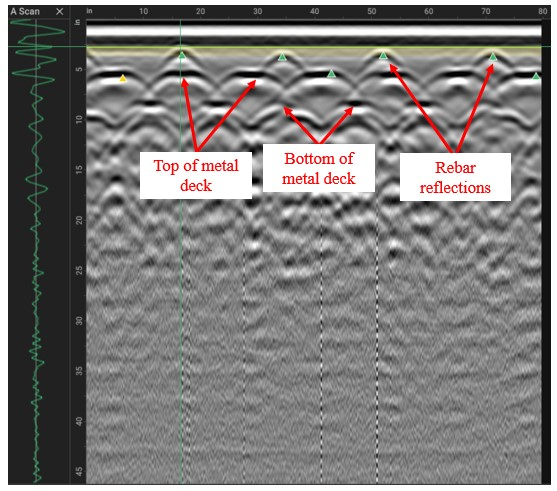
\includegraphics[width=\linewidth, height=0.65\linewidth]{img/gpr_radargram.jpg}
      \captionof{figure}{GPR B-scan: hyperbolic rebar echoes}
      \label{fig:radargram}
    \end{minipage}\hfill%
    \begin{minipage}[t]{0.48\linewidth}
      \centering
      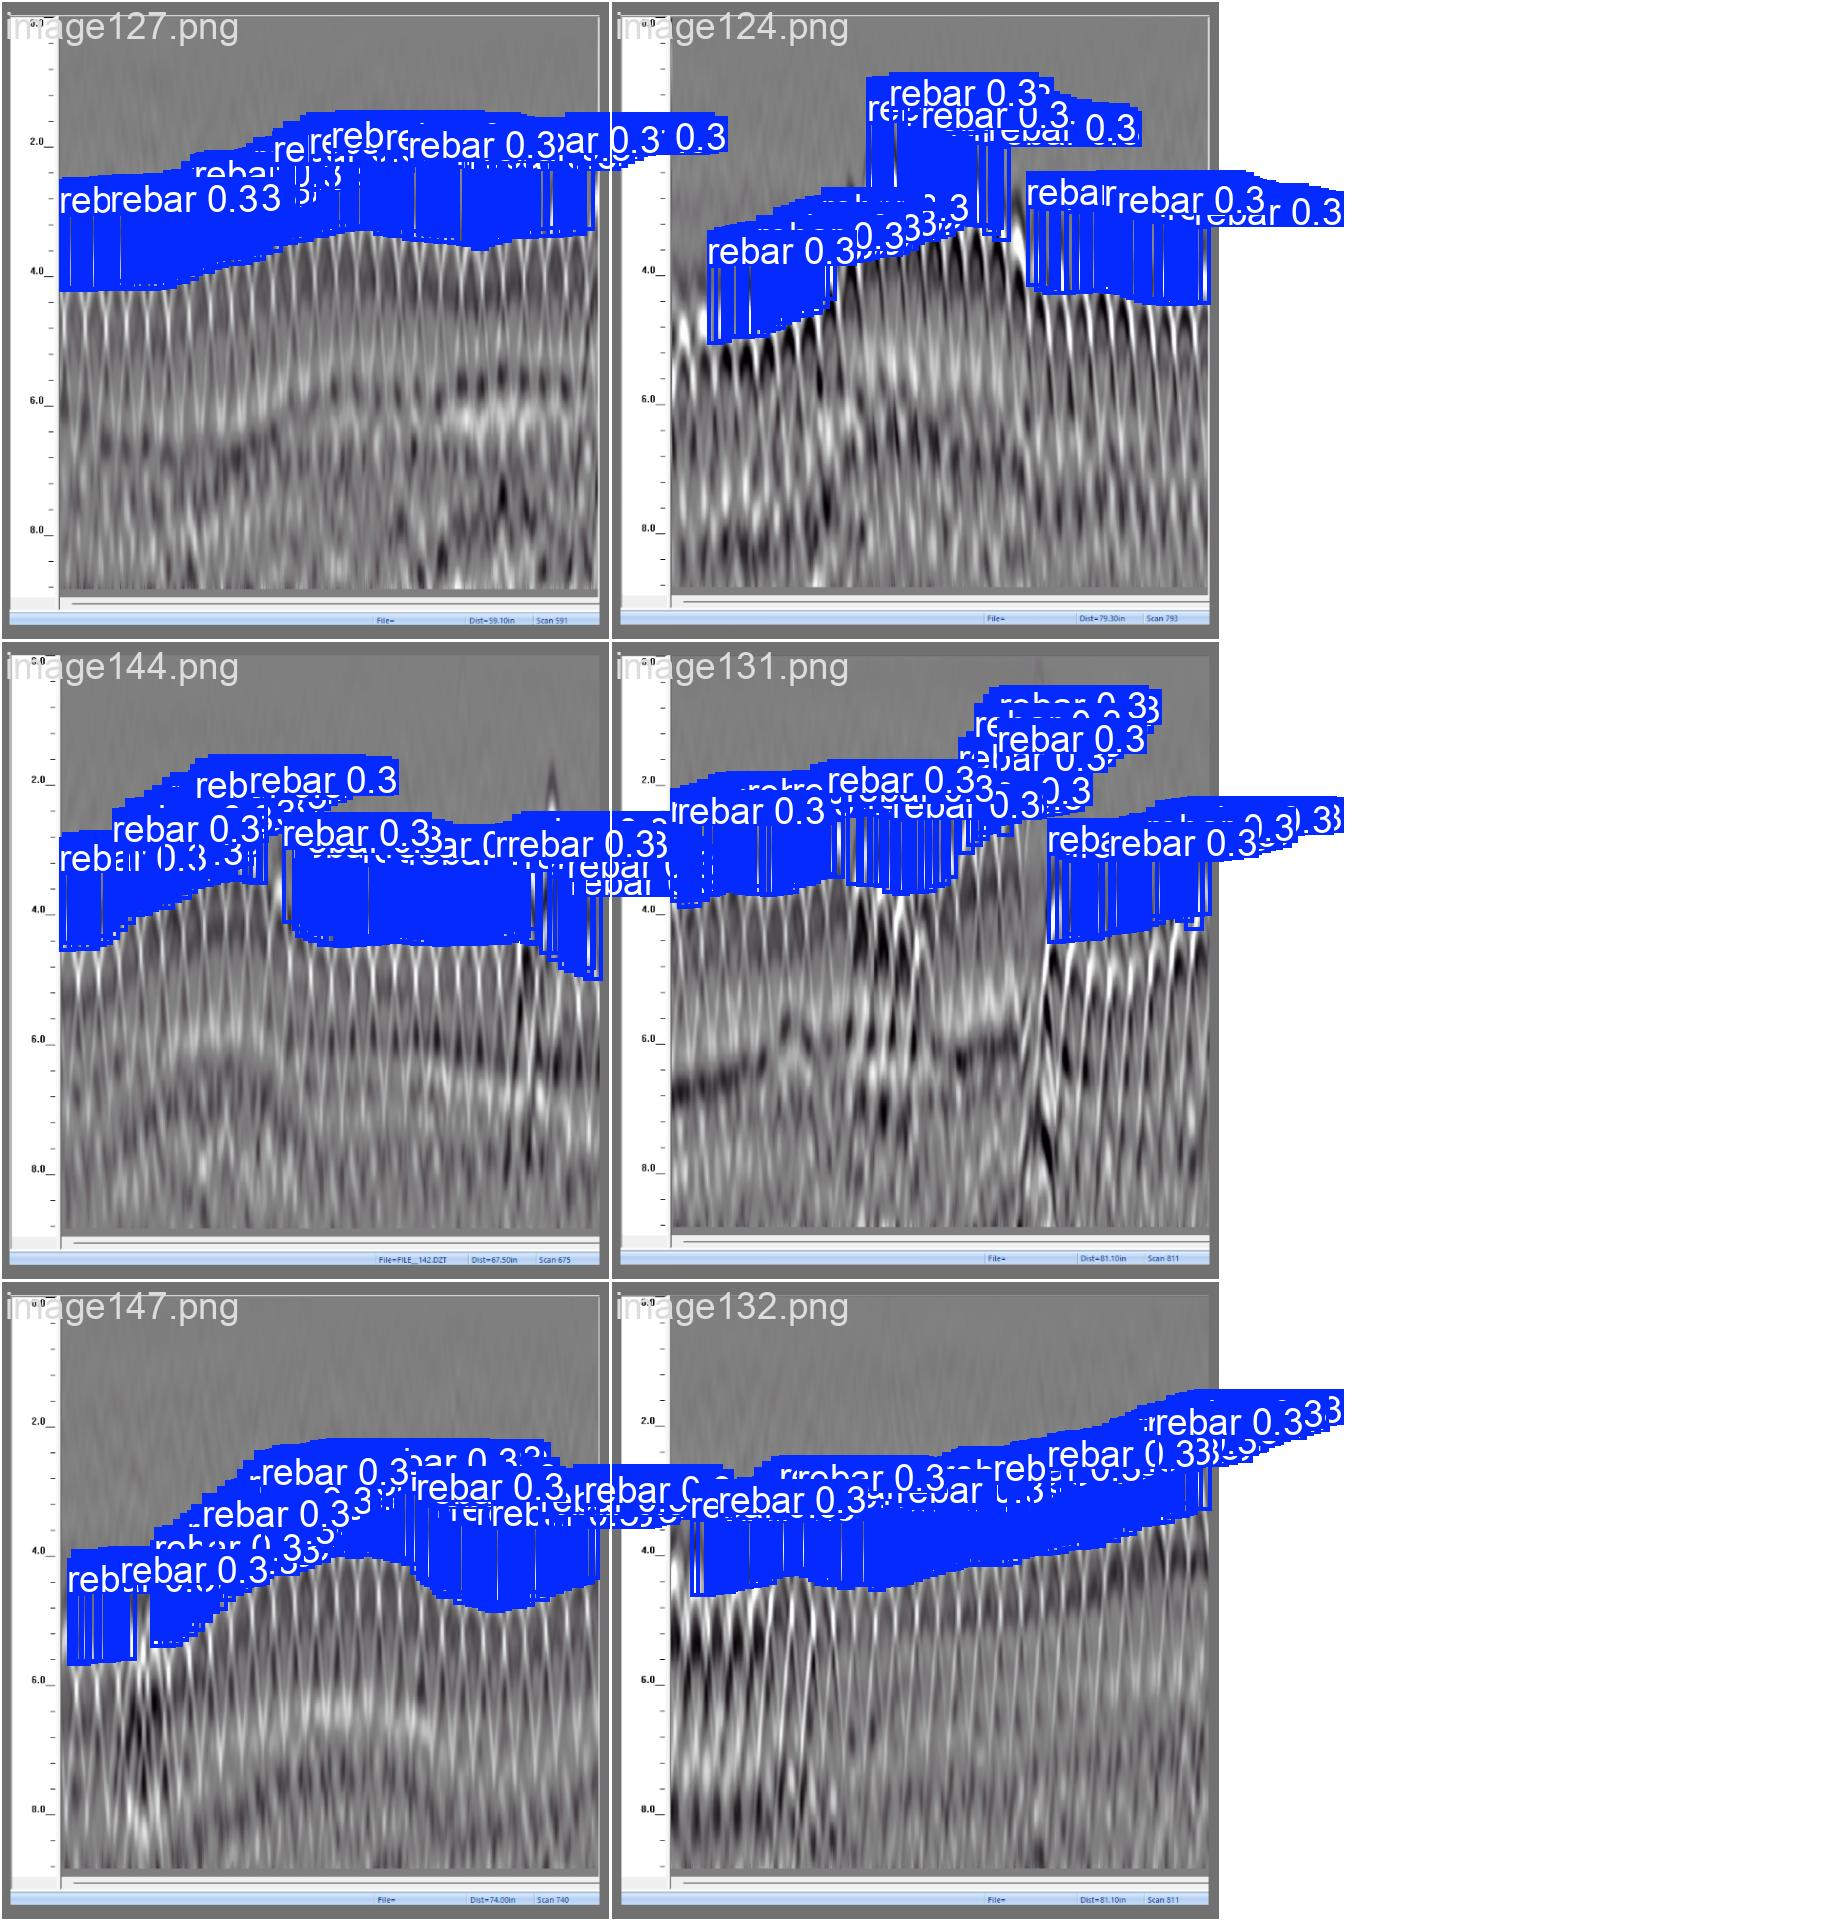
\includegraphics[width=\linewidth, height=0.65\linewidth]{img/gssi_predictions.jpg}
      \captionof{figure}{GSSI SIR-3000 YOLOv8n detections}
      \label{fig:gssi-pred}
    \end{minipage}

    \vspace{0.75cm}

    \noindent\begin{minipage}[t]{\linewidth}
      \centering
      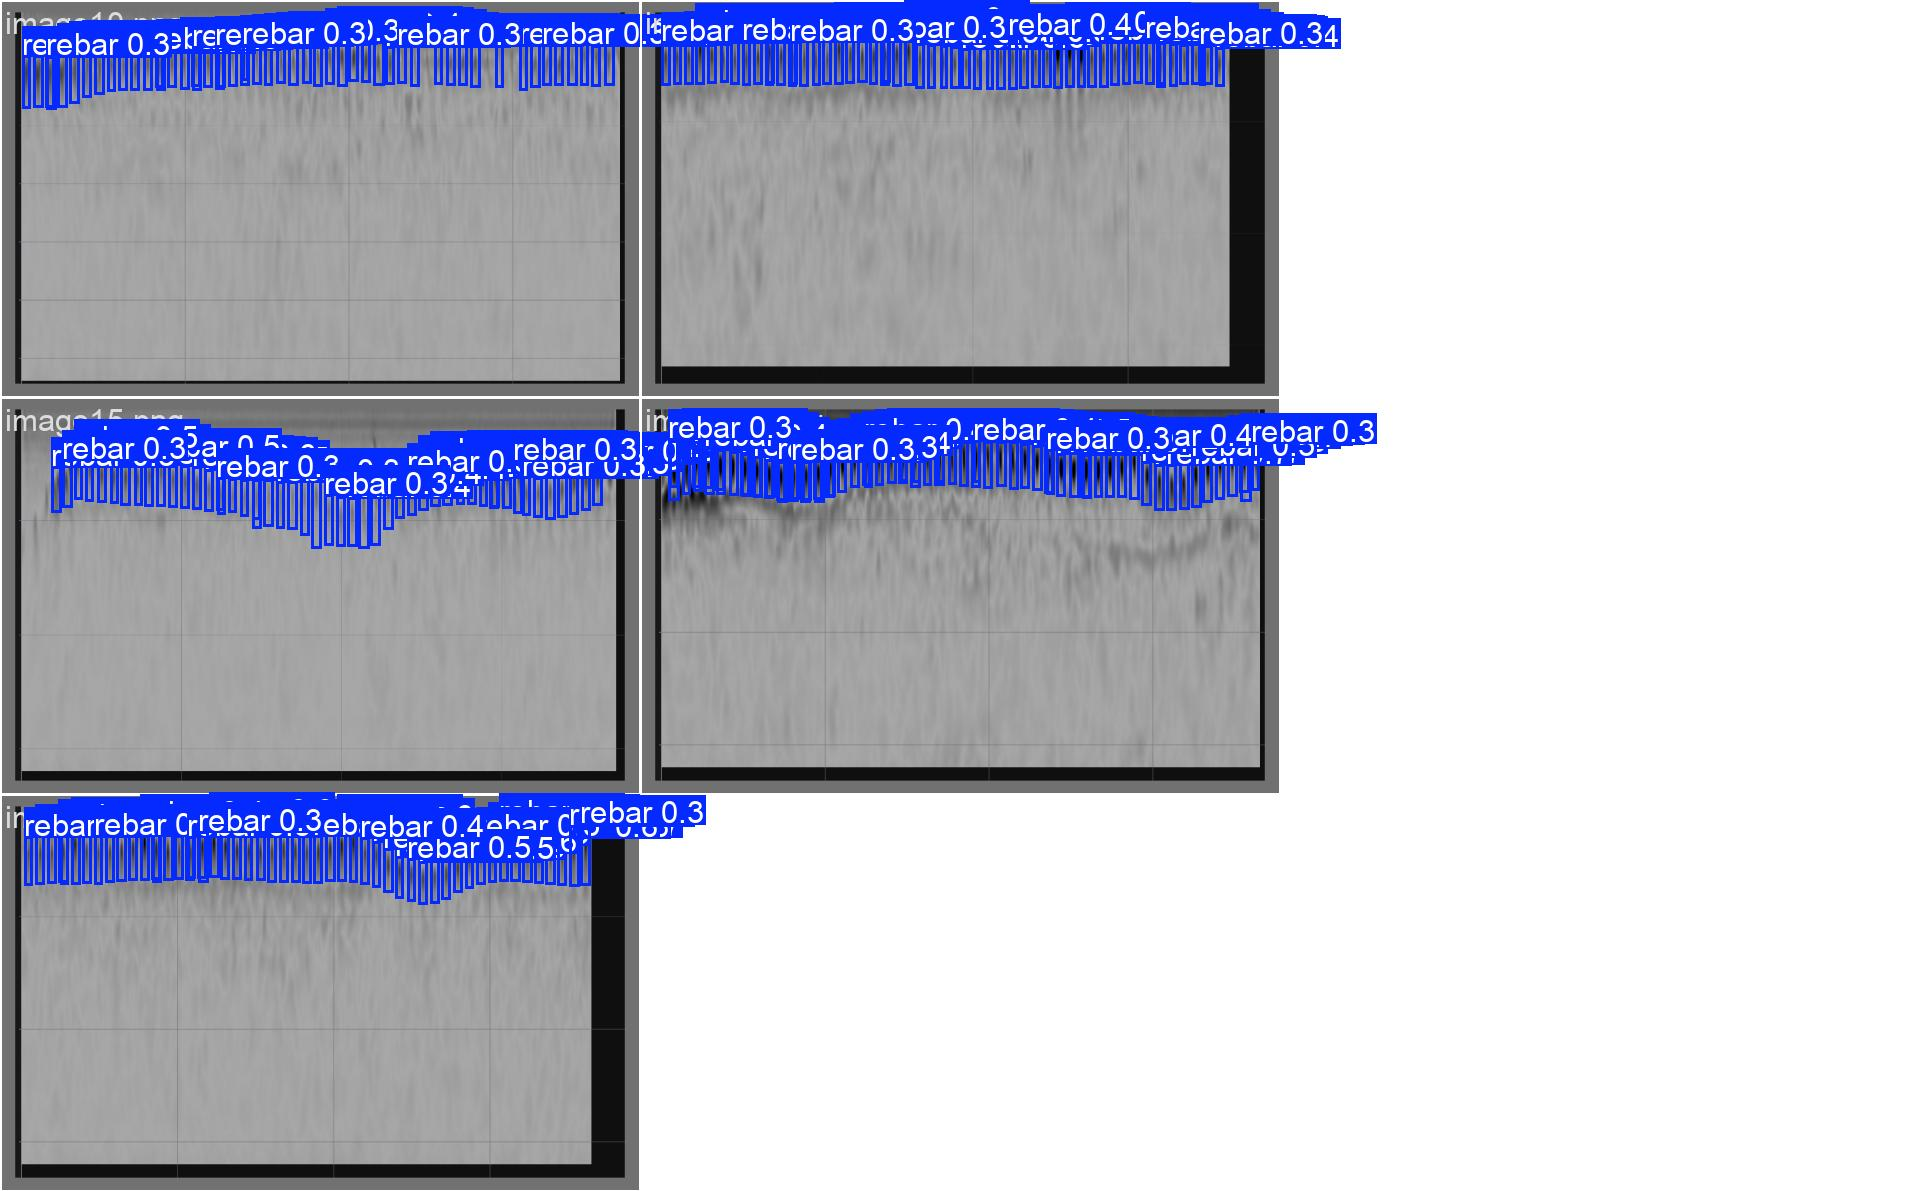
\includegraphics[width=\linewidth, height=0.45\linewidth]{img/gp8000_predictions.jpg}
      \captionof{figure}{GP8000 YOLOv8n detections on bridge-deck B-scan data}
      \label{fig:gp8000-pred}
    \end{minipage}

    Annotations were created in CVAT on B-scans from Georgia Southern ERB bridge decks and Georgia DOT field data, covering both scanner hardware types.

    \header{Problem Statement}[0pt]

    \vspace{0.5cm}

    No existing open-source pipeline performs \textbf{hardware-adaptive} rebar detection across GPR platforms. Both the GSSI SIR-3000 and the GP8000 produce structurally different radargrams, and a single model trained on one scanner generalizes poorly to the other.

    This leads us to the core research question: \emph{Can a YOLOv8n model fine-tuned per hardware platform achieve production-grade rebar detection on bridge-deck GPR data?} Such a system could reduce inspection costs, enable field deployment on commodity hardware, and support the Georgia DOT's bridge management workflow.

    \vspace{0.5cm}

    \noindent\begin{minipage}[t]{0.48\linewidth}
      \centering
      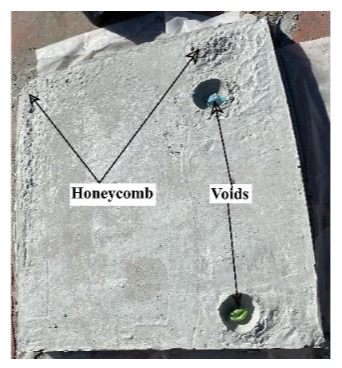
\includegraphics[width=\linewidth, height=0.75\linewidth]{img/defect_honeycomb.png}
      \captionof{figure}{Honeycombing \& voids in concrete}
    \end{minipage}\hfill
    \begin{minipage}[t]{0.48\linewidth}
      \centering
      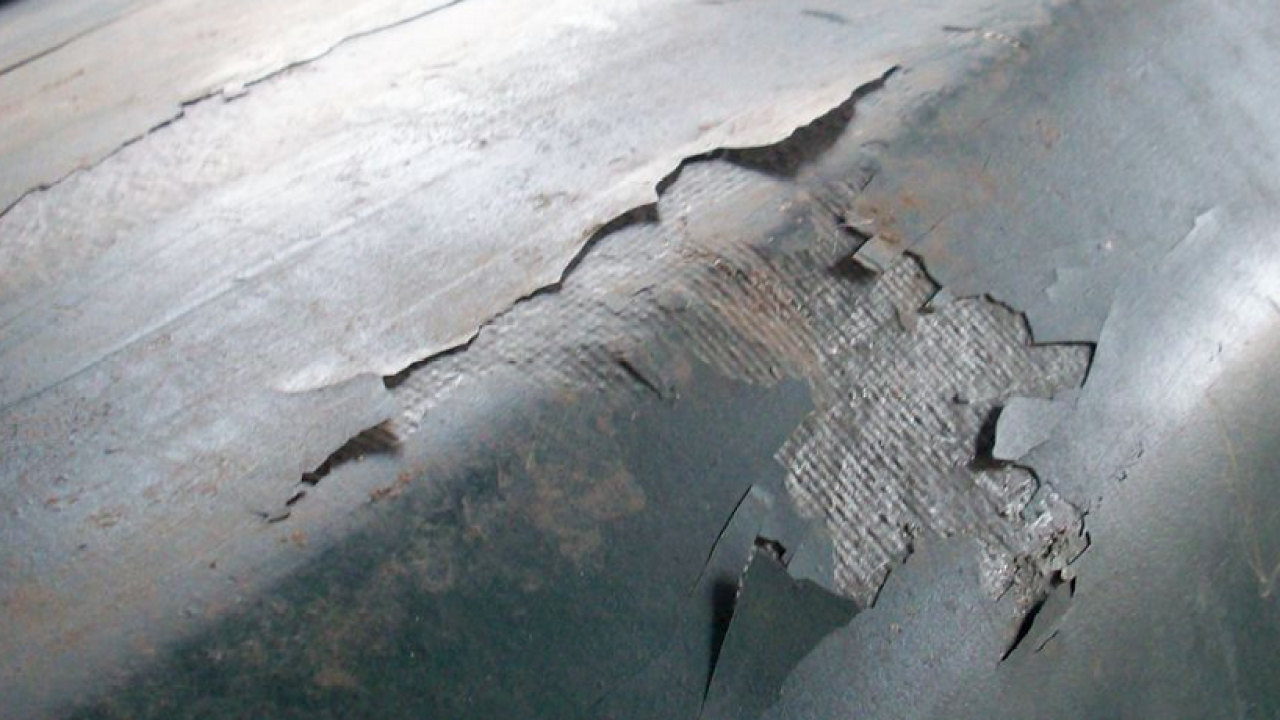
\includegraphics[width=\linewidth, height=0.75\linewidth]{img/defect_spalling.png}
      \captionof{figure}{Concrete spalling / delamination}
    \end{minipage}

    \vspace{0.5cm}

    \noindent\begin{minipage}[t]{0.48\linewidth}
      \centering
      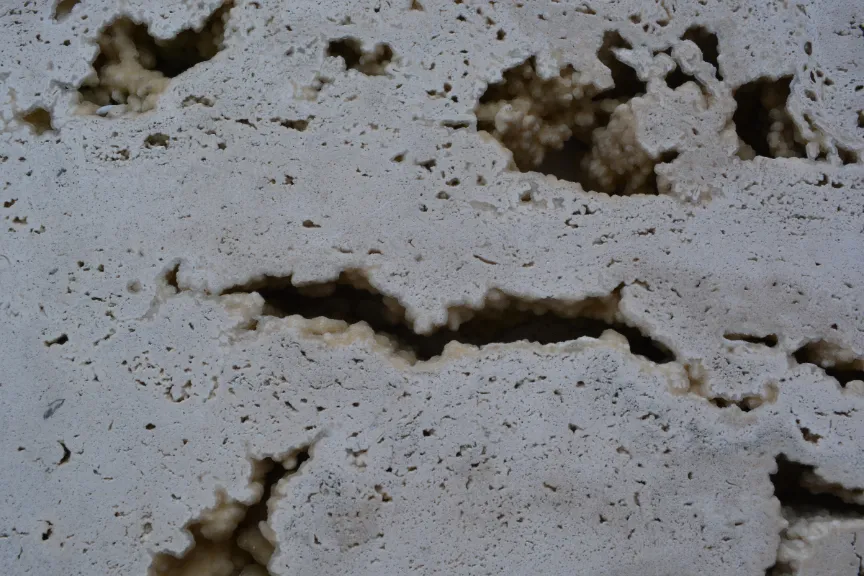
\includegraphics[width=\linewidth, height=0.75\linewidth]{img/defect_cracking.png}
      \captionof{figure}{Surface cracking \& deterioration}
    \end{minipage}\hfill
    \begin{minipage}[t]{0.48\linewidth}
      \centering
      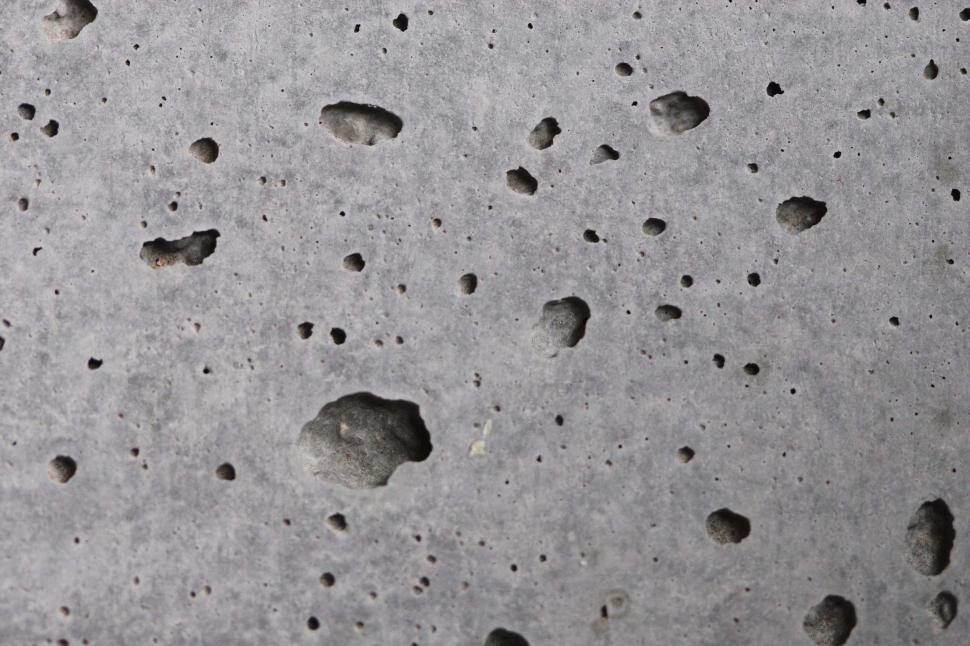
\includegraphics[width=\linewidth, height=0.75\linewidth]{img/defect_voids.png}
      \captionof{figure}{Subsurface void pitting}
    \end{minipage}

    \vspace{0.5cm}

  \end{block}

  \begin{block}{Hypothesis \& Objectives}

    \header{Hypothesis}[0pt]

    \vspace{0.5cm}

    A YOLOv8n model fine-tuned on hardware-specific GPR data achieves mAP@0.5 $\geq$ 0.75 on structured bridge-deck B-scans.

    \header{Objectives}[0pt]

    \vspace{0.5cm}

    \begin{itemize}
      \item Train \textbf{YOLOv8n} separately for GSSI SIR-3000 and GP8000 scanner data
      \item Release first \textbf{public GPR rebar annotation dataset}
      \item Benchmark vs.\ RetinaNet, Faster-RCNN, Wetectron, PCL, C-MIL
      \item Deploy \textbf{desktop GUI} for Georgia DOT field engineers
    \end{itemize}

    \vspace{0.5cm}

    \begin{minipage}[t]{\linewidth}
      \centering
      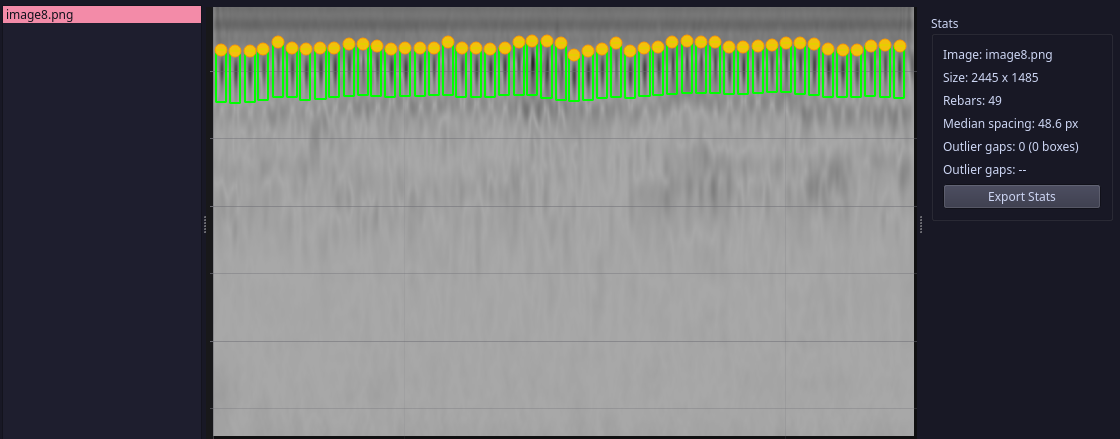
\includegraphics[width=\linewidth]{img/App.png}
      \captionof{figure}{ConcreteNet desktop application: real-time GPR rebar detection GUI}
      \label{fig:app-screenshot}
    \end{minipage}

    \vspace{0.5cm}

  \end{block}

\end{column}

\separatorcolumn

\begin{column}{\twocolwidth}

  \begin{block}{Methodology or Approach}

    \header{Inference Pipeline}[0pt]

    \vspace{1cm}

    \begin{minipage}{0.24\linewidth}
      \subheader{Data Sources}
      \begin{itemize}
        \item GSSI SIR-3000 scanner
        \item Leica GP8000 scanner
        \item GSU ERB floor scans
        \item Georgia DOT field B-scans (anticipated)
        \item Annotated in CVAT
      \end{itemize}
    \end{minipage}\hfill%
    \begin{minipage}{0.72\linewidth}
      \subheader{Training Configuration}
      \begin{multicols}{3}
      \begin{description}
        \item[Model] YOLOv8n
        \item[Input] $640\times640$ px
        \item[Epochs] 300
        \item[Batch] 16
        \item[Optimizer] AdamW
        \item[LR] $10^{-3}$
        \item[NMS IoU] 0.45
        \item[Conf. Threshold] 0.25
        \item[Augmentation] Mosaic, HSV
        \item[Hardware] NVIDIA GPU
        \item[Framework] Ultralytics
        \item[Classes] rebar, void
      \end{description}
    \end{multicols}
    \end{minipage}

    \header{Experimental Setup}

    \begin{minipage}[t]{0.48\linewidth}
      \subheader{GSSI SIR-3000 Pipeline}
      \begin{enumerate}
        \item Collect raw B-scan data from bridge decks
        \item Export to DZT format and convert to PNG strips
        \item Annotate hyperbolic rebar echoes in CVAT
        \item Split 70/20/10 train/val/test
        \item Fine-tune YOLOv8n for 300 epochs
        \item Evaluate mAP@0.5, Precision, Recall on held-out test set
        \item Export model weights for GUI deployment
      \end{enumerate}

      \vspace{1cm}

      \begin{figure}[H]
        \centering
        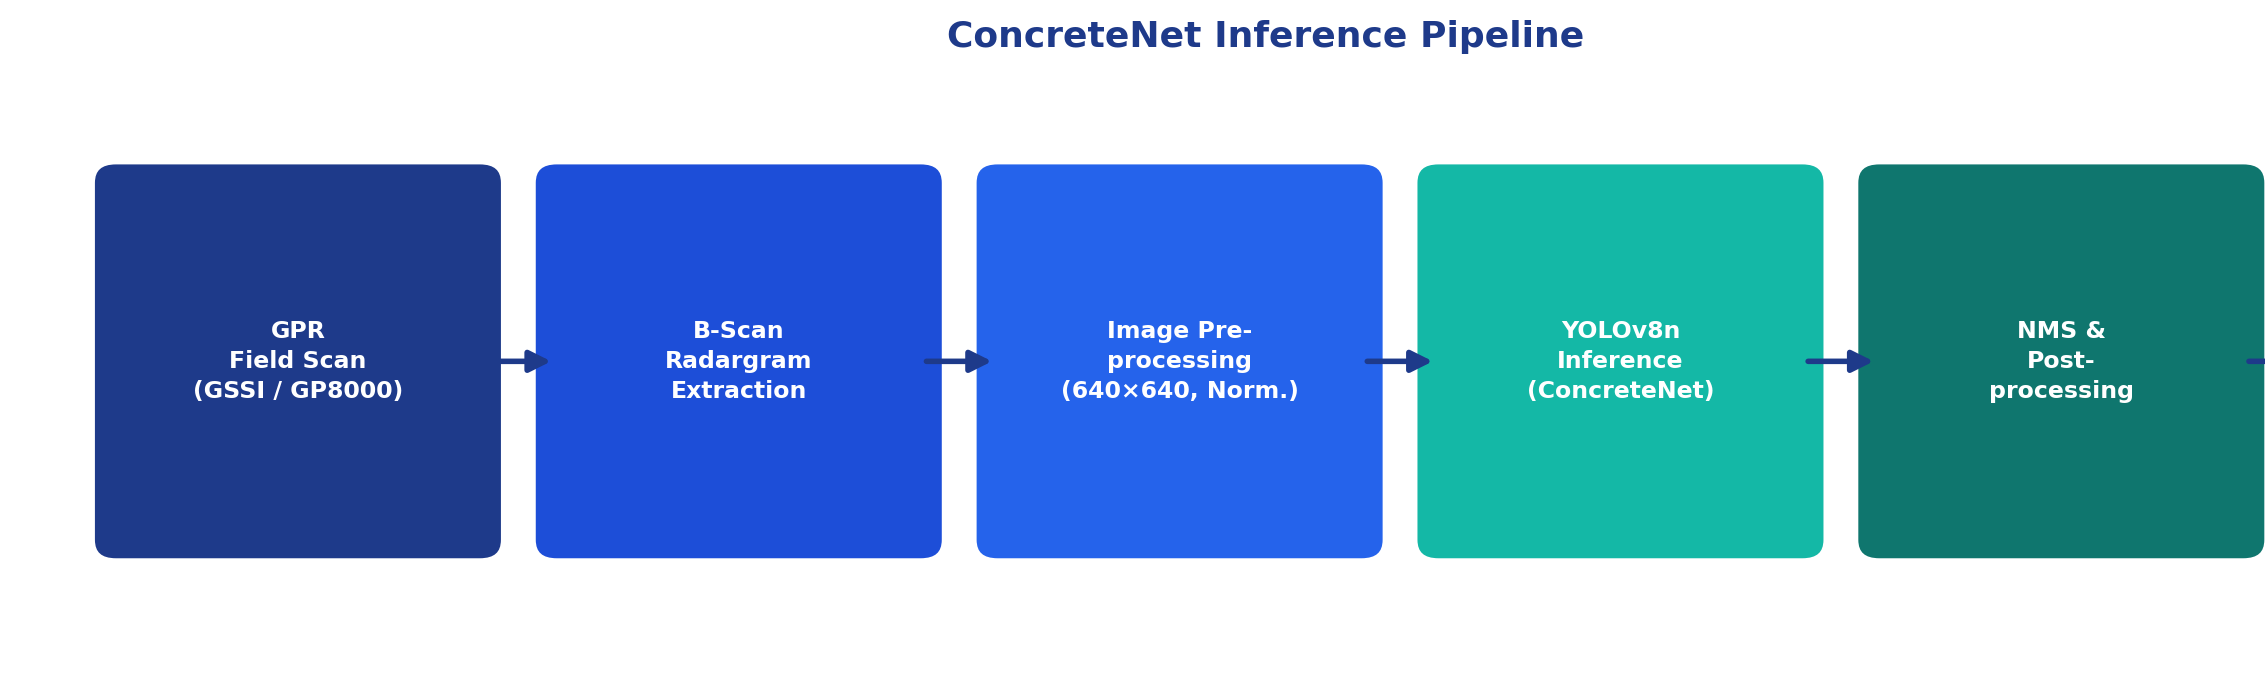
\includegraphics[width=0.97\linewidth, height=0.35\linewidth]{img/pipeline.png}
        \caption{Inference pipeline from raw B-scan to annotated output}
        \label{fig:pipeline}
      \end{figure}

    \end{minipage}\hfill%
    \begin{minipage}[t]{0.48\linewidth}
      \subheader{GP8000 Pipeline}

      \begin{enumerate}
        \item Same data collection procedure as GSSI
        \item Export GP8000 proprietary format to PNG
        \item Re-annotate due to different scan resolution/scale
        \item Train separate YOLOv8n model (no weight sharing)
        \item Evaluate on GP8000-specific test set
        \item Compare cross-hardware mAP to quantify domain gap
        \item Package both models in ConcreteNet GUI
      \end{enumerate}

      \vspace{1cm}

      \begin{figure}[H]
        \centering
         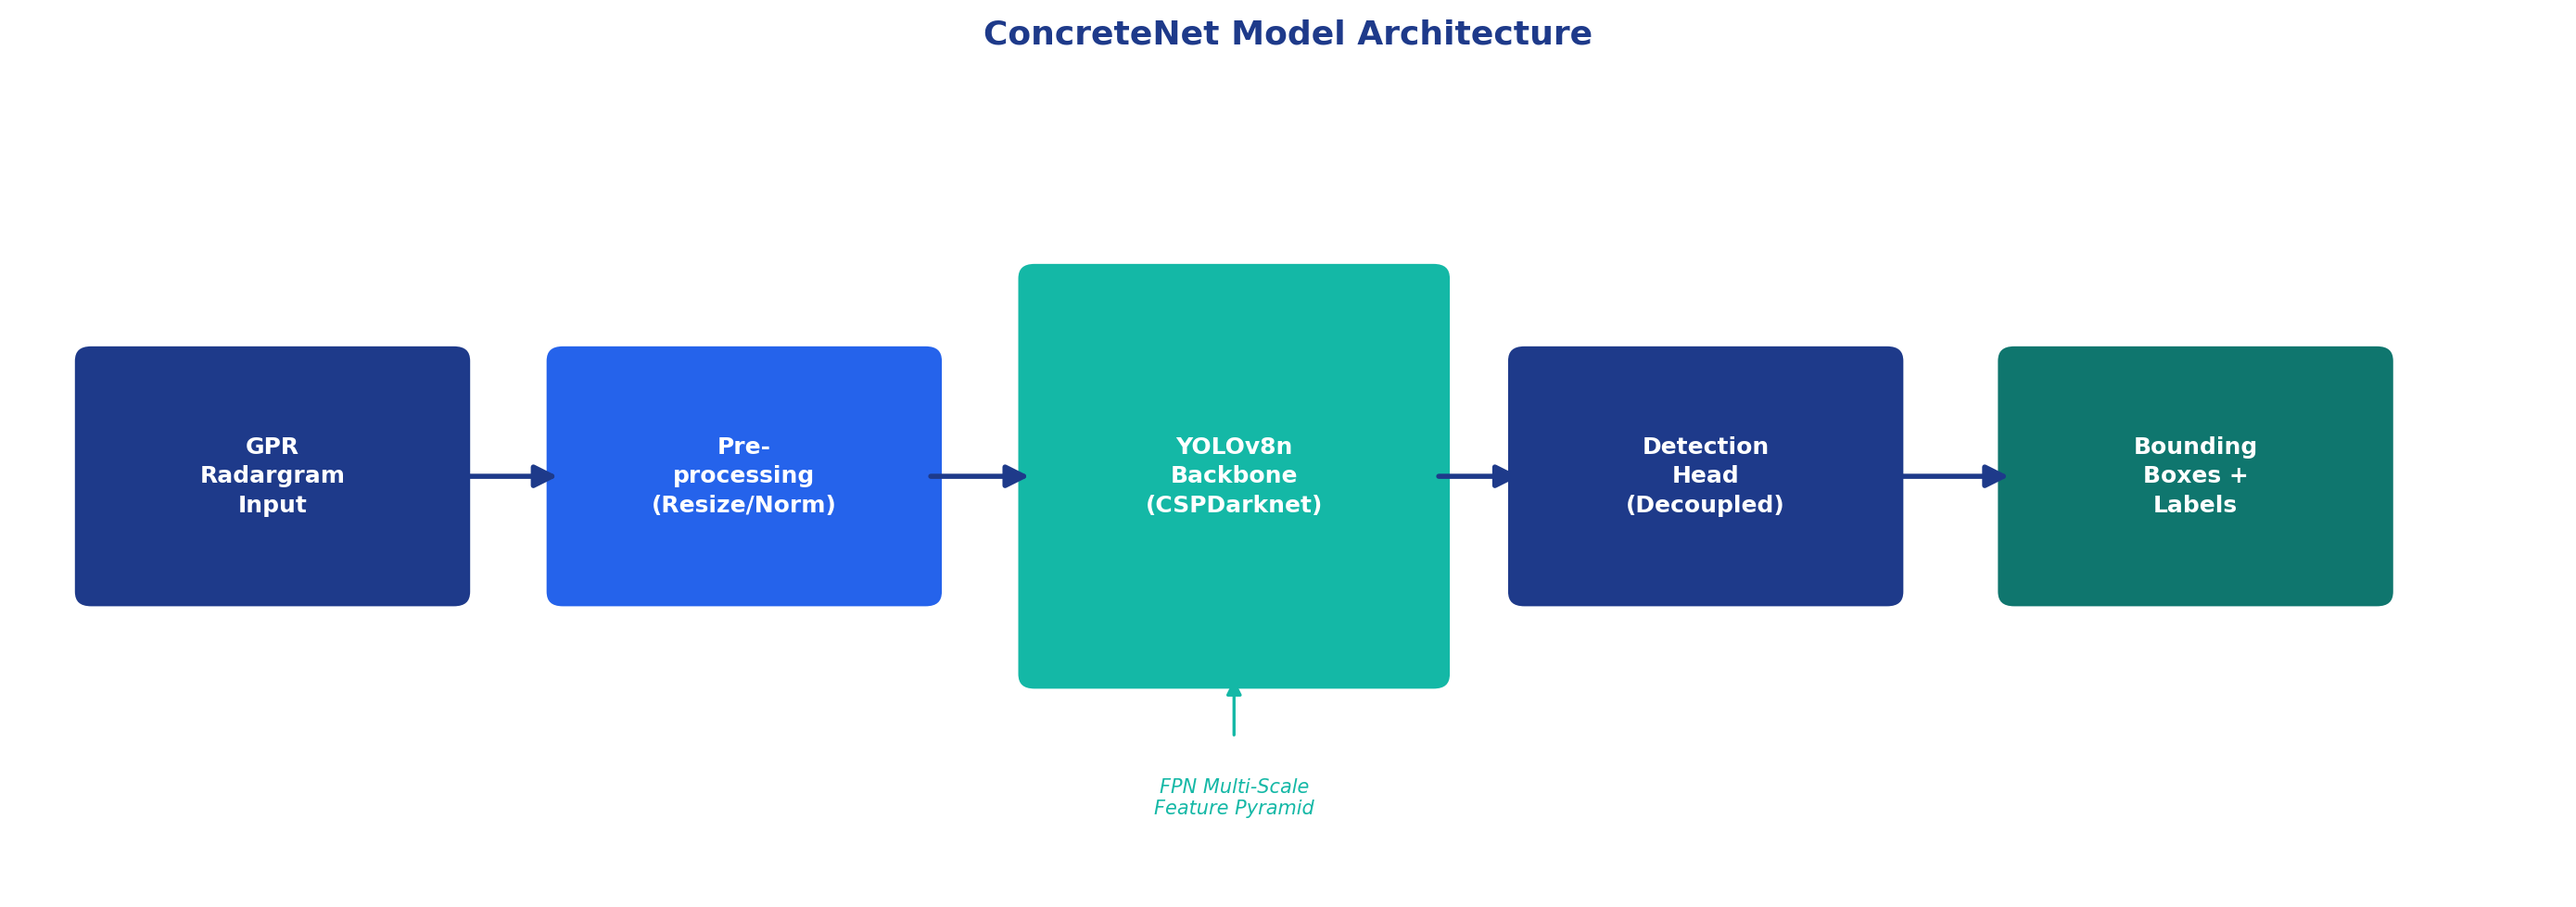
\includegraphics[height=0.5\linewidth, width=0.9\linewidth]{img/architecture.png}
         \caption{YOLOv8n architecture: CSPDarknet backbone, C2f neck, decoupled head}
         \label{fig:architecture}
       \end{figure}
    \end{minipage}

    \vspace*{1cm}

    \header{Model Architecture}[0pt]

    \begin{minipage}[t]{0.48\linewidth}
      \subheader{YOLOv8n Backbone}

      YOLOv8n uses a \textbf{CSPDarknet + C2f} backbone with FPN multi-scale feature extraction at strides 8, 16, and 32. A \textbf{decoupled detection head} separates classification and regression branches, reducing task interference.

      \vspace{1cm}
      Combined training loss:
      \begin{align*}
        \mathcal{L} &= \lambda_1 \mathcal{L}_\text{box} + \lambda_2 \mathcal{L}_\text{cls} + \lambda_3 \mathcal{L}_\text{dfl}
      \end{align*}
      where $\lambda_1=7.5$, $\lambda_2=0.5$, $\lambda_3=1.5$. Distribution Focal Loss:
      \begin{align*}
        \mathcal{L}_\text{dfl} = -\!\sum_{i}\bigl[(1-p_i)\log p_i + p_i\log(1-p_i)\bigr]
      \end{align*}
      AdamW: $lr = 10^{-3}$, batch $= 16$, NMS IoU $= 0.45$.

      \vspace{1cm}

    \end{minipage}\hfill%
    \begin{minipage}[t]{0.48\linewidth}
      \subheader{ConcreteNet GUI}

      The \textbf{ConcreteNet desktop application} is a field-deployable PyQt5 GUI that runs both trained models without requiring a Python environment setup. Features include one-click inference on B-scan images, bounding-box overlay editing, rebar spacing analysis, and PNG/PDF export. Engineers select the scanner type and the appropriate model weights load automatically.

      \vspace{1cm}

      \begin{figure}[H]
        \centering
        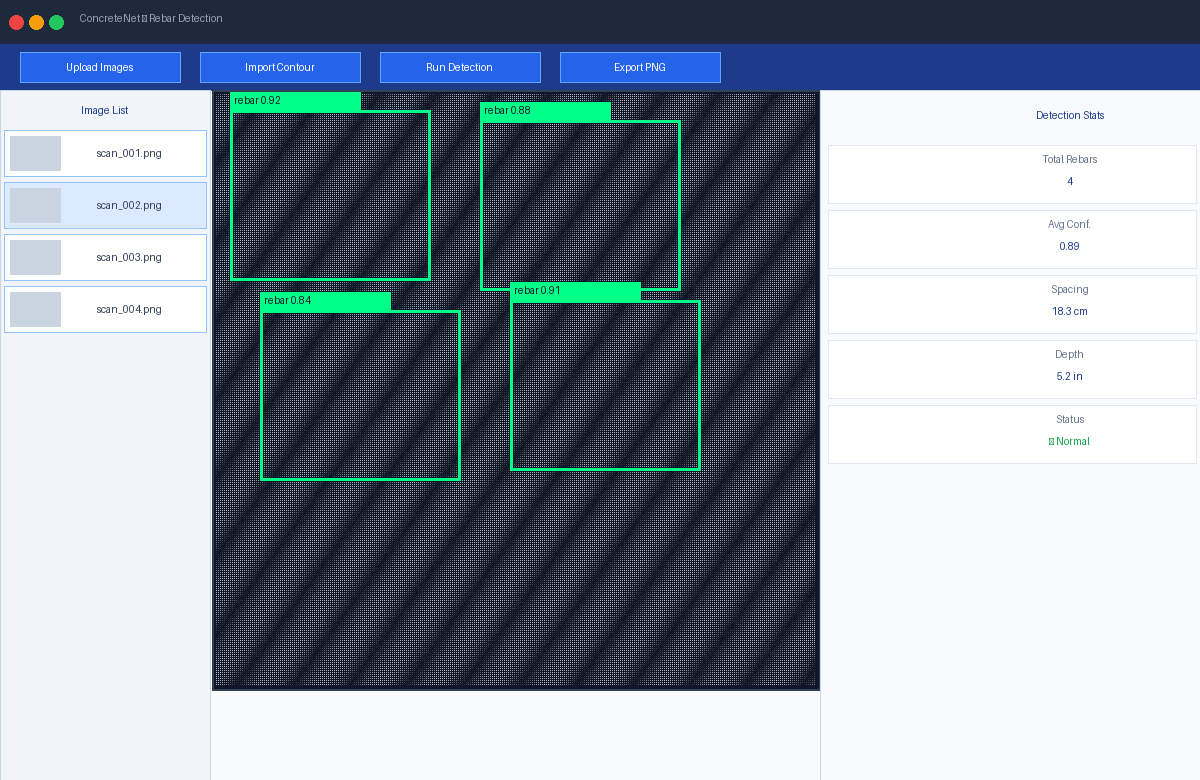
\includegraphics[width=0.95\linewidth]{img/app_mockup.png}
        \caption{ConcreteNet GUI: annotated canvas with real-time stats}
        \label{fig:app}
      \end{figure}
    \end{minipage}

    \header{Performance Results}[0pt]

    \vspace{0.5cm}

    % Training Curves row
    \subheader{Training Curves}
    \vspace{0.4cm}

    \noindent\begin{minipage}[t]{0.48\linewidth}
      \centering
      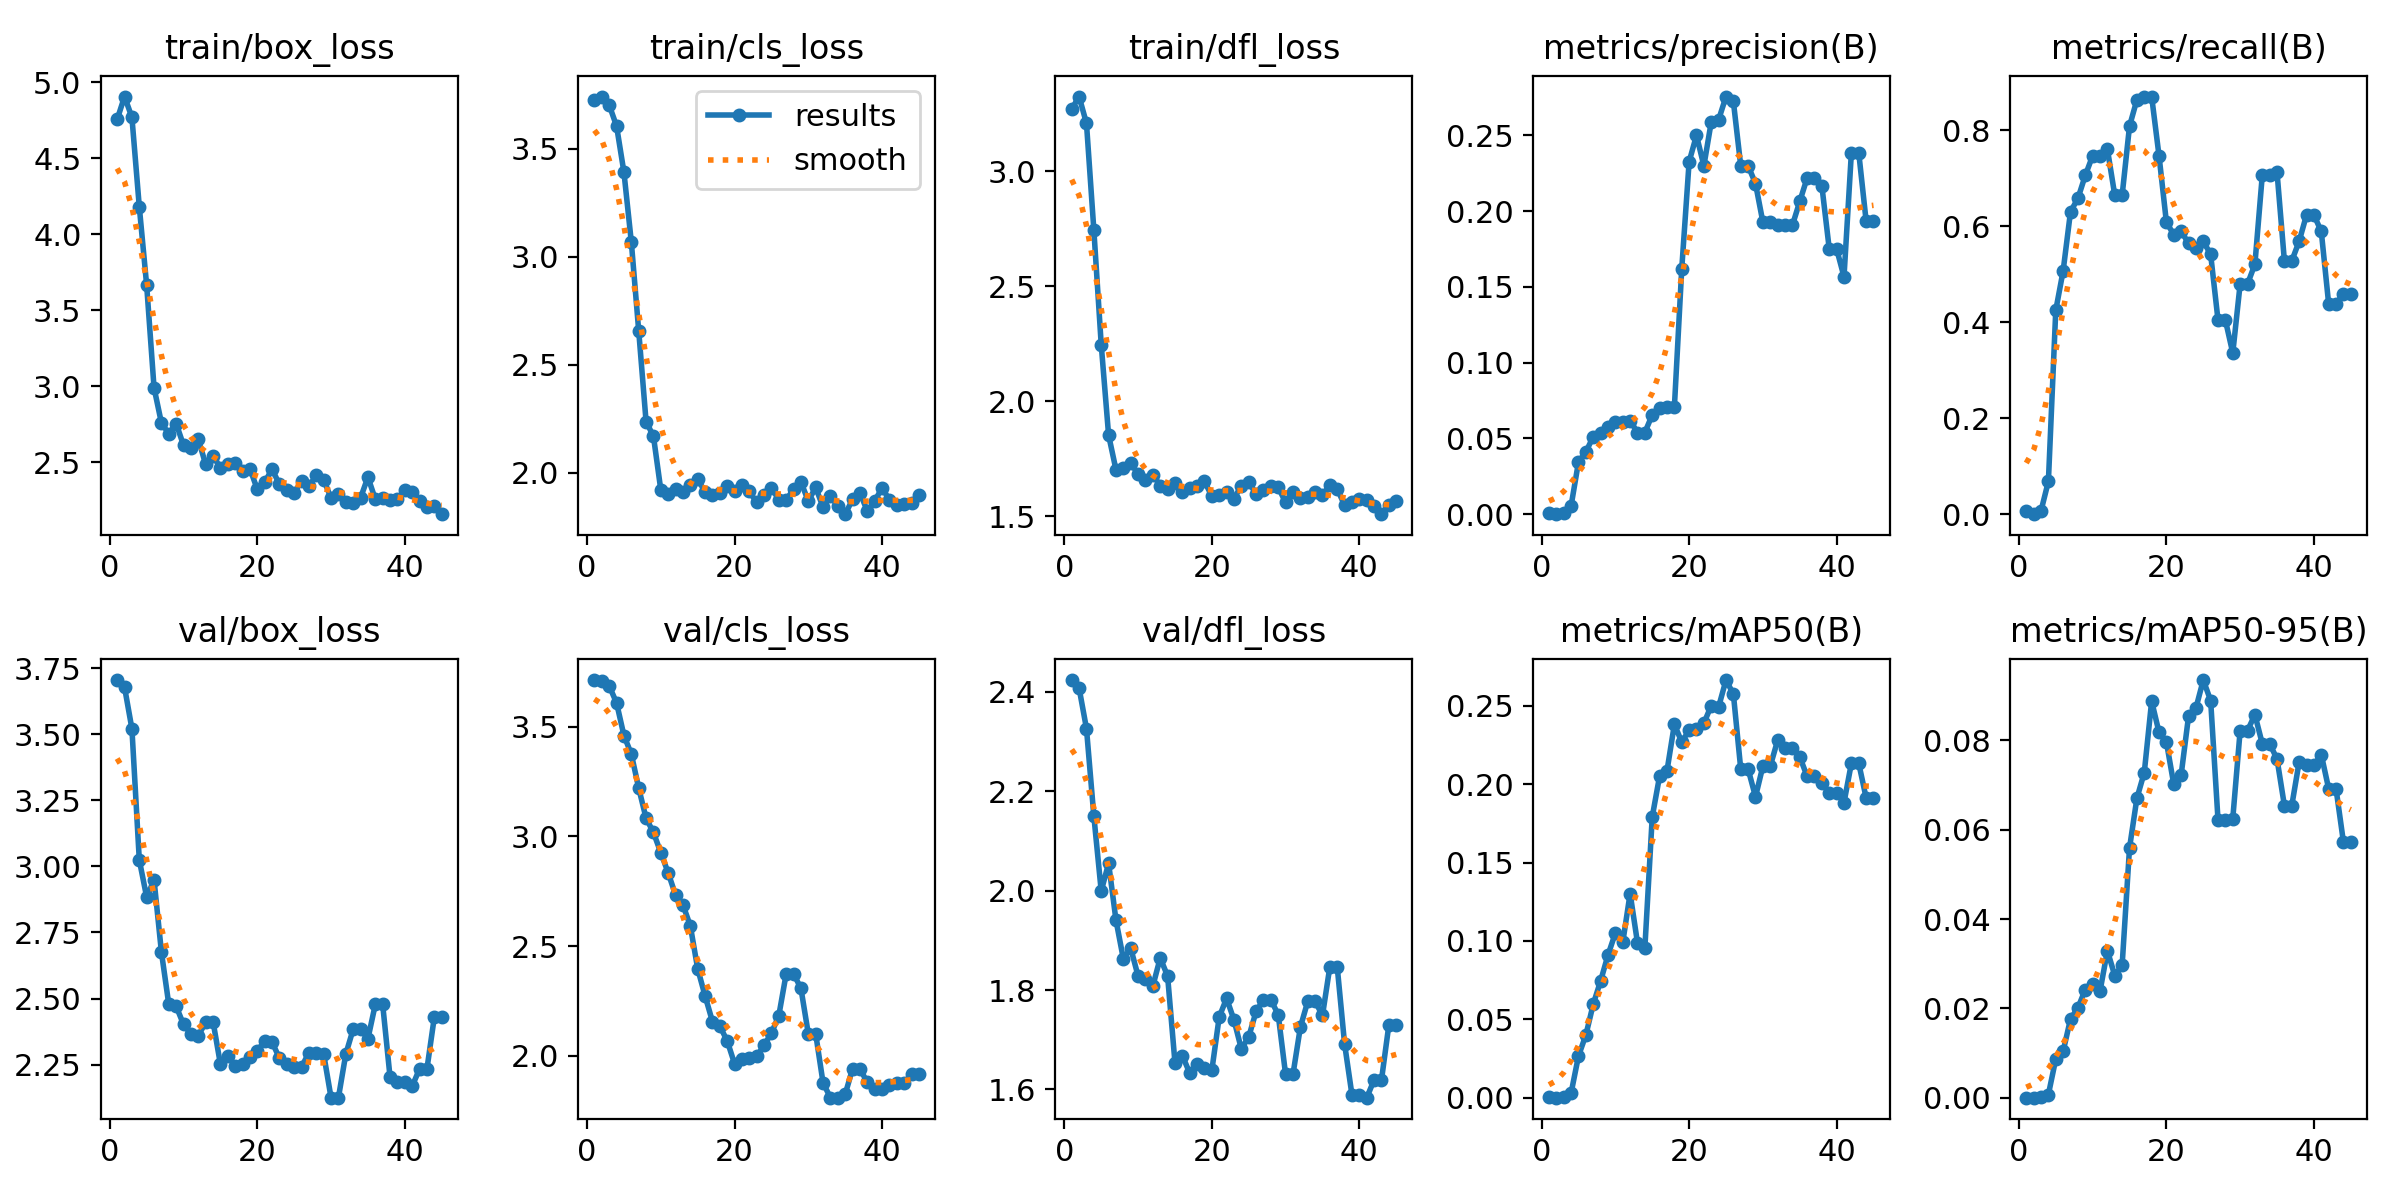
\includegraphics[width=\linewidth]{img/gssi_results.png}
      \captionof{figure}{GSSI training metrics}
      \label{fig:gssi-results}
    \end{minipage}\hfill
    \begin{minipage}[t]{0.48\linewidth}
      \centering
      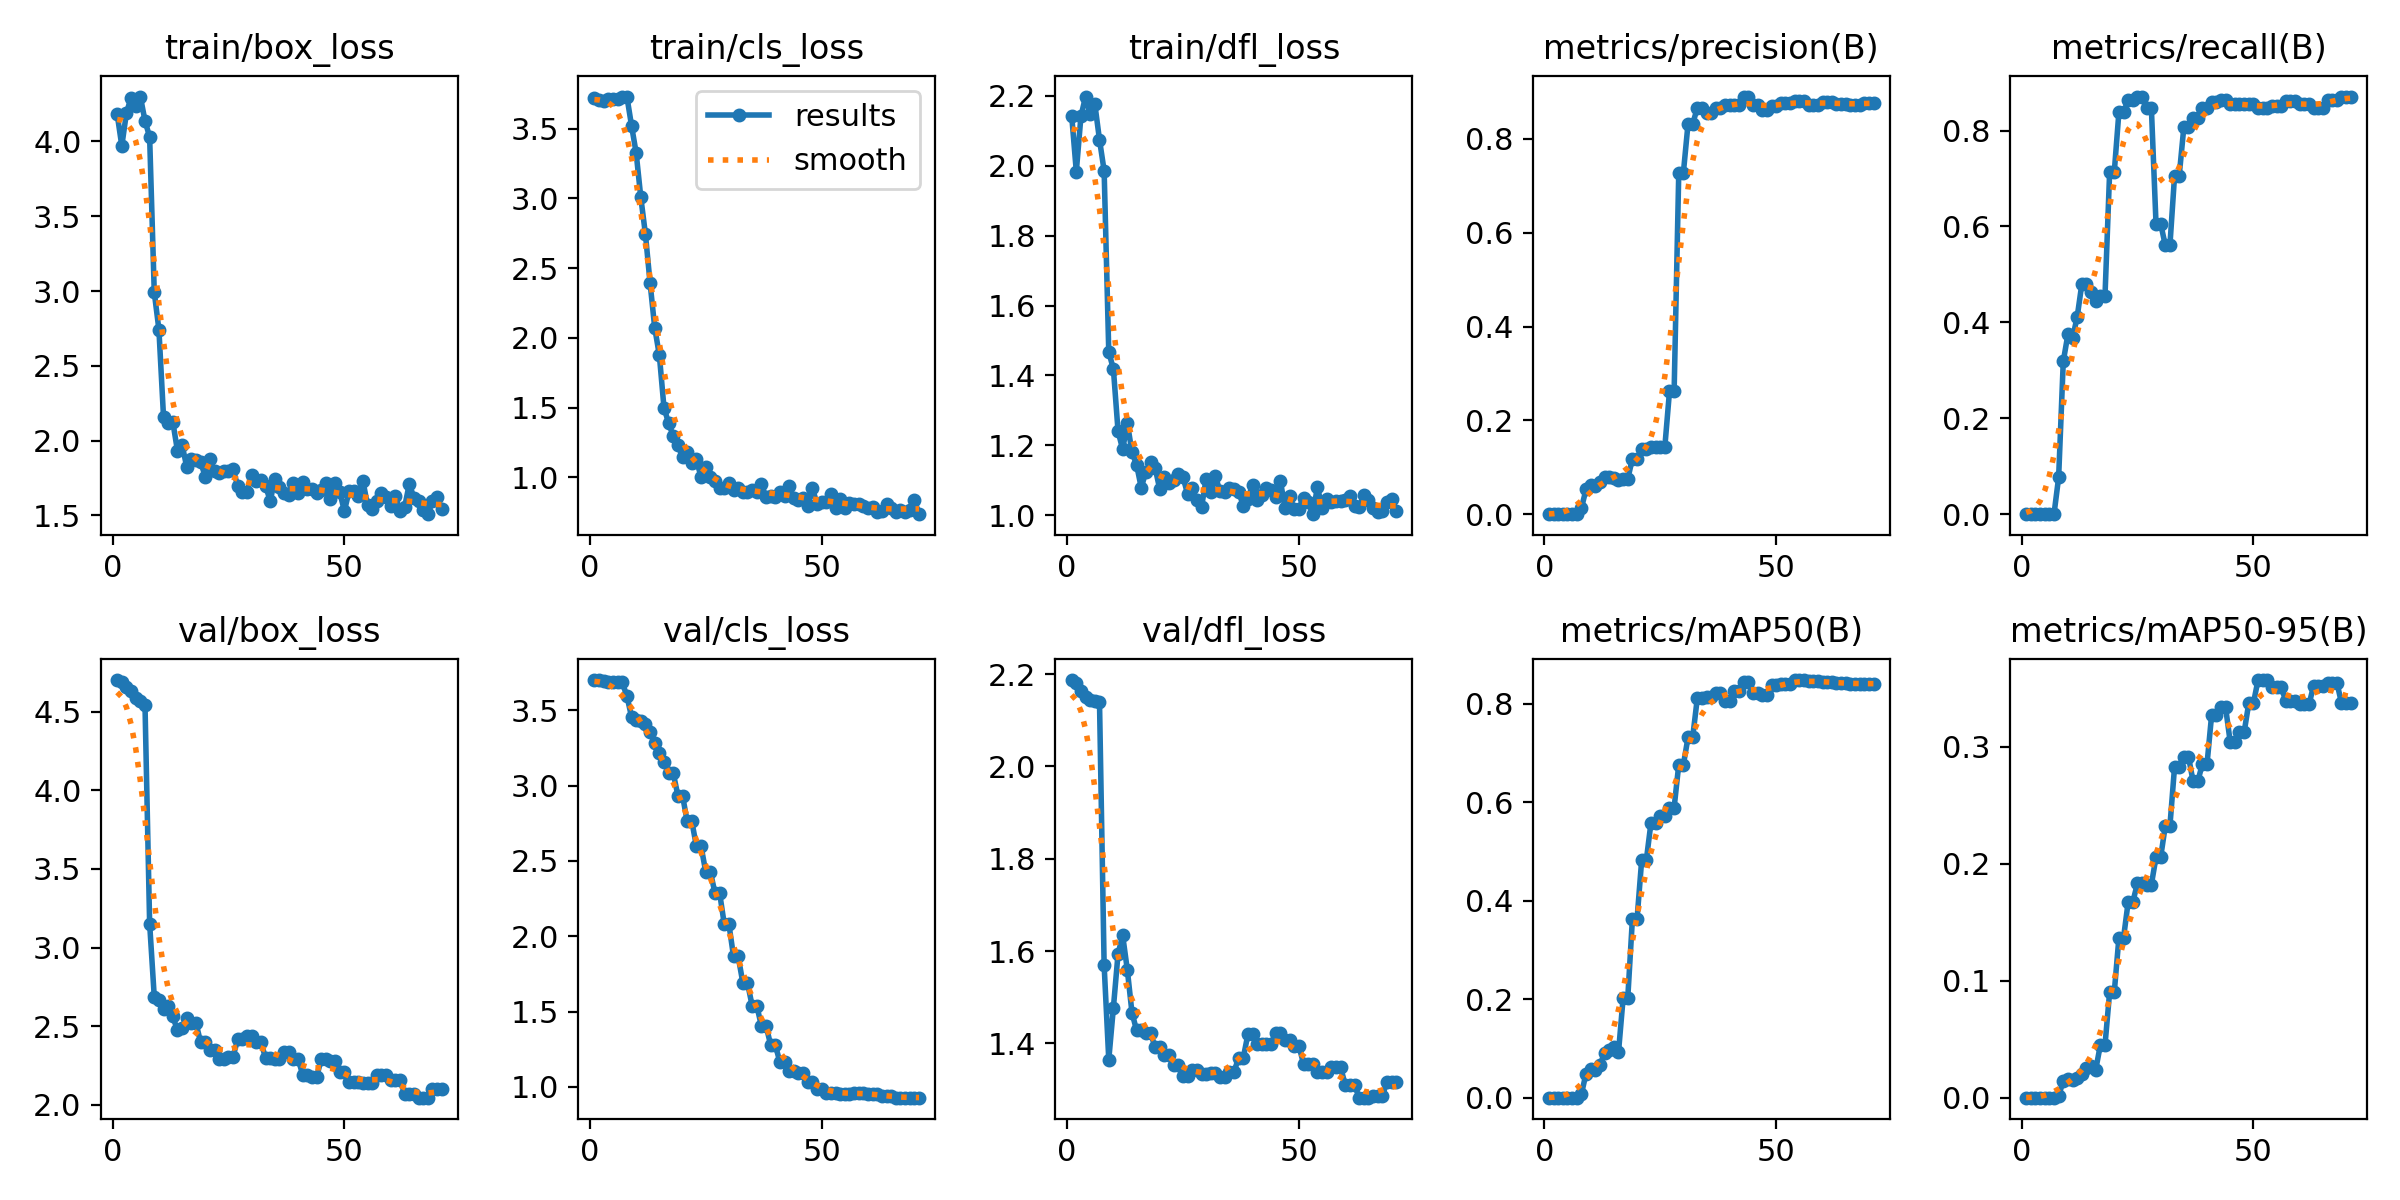
\includegraphics[width=\linewidth]{img/gp8000_results.png}
      \captionof{figure}{GP8000 training metrics}
      \label{fig:gp8000-results}
    \end{minipage}

    \vspace{0.75cm}

    % PR Curves row
    \subheader{PR Curves}
    \vspace{0.4cm}

    \noindent\begin{minipage}[t]{0.48\linewidth}
      \centering
      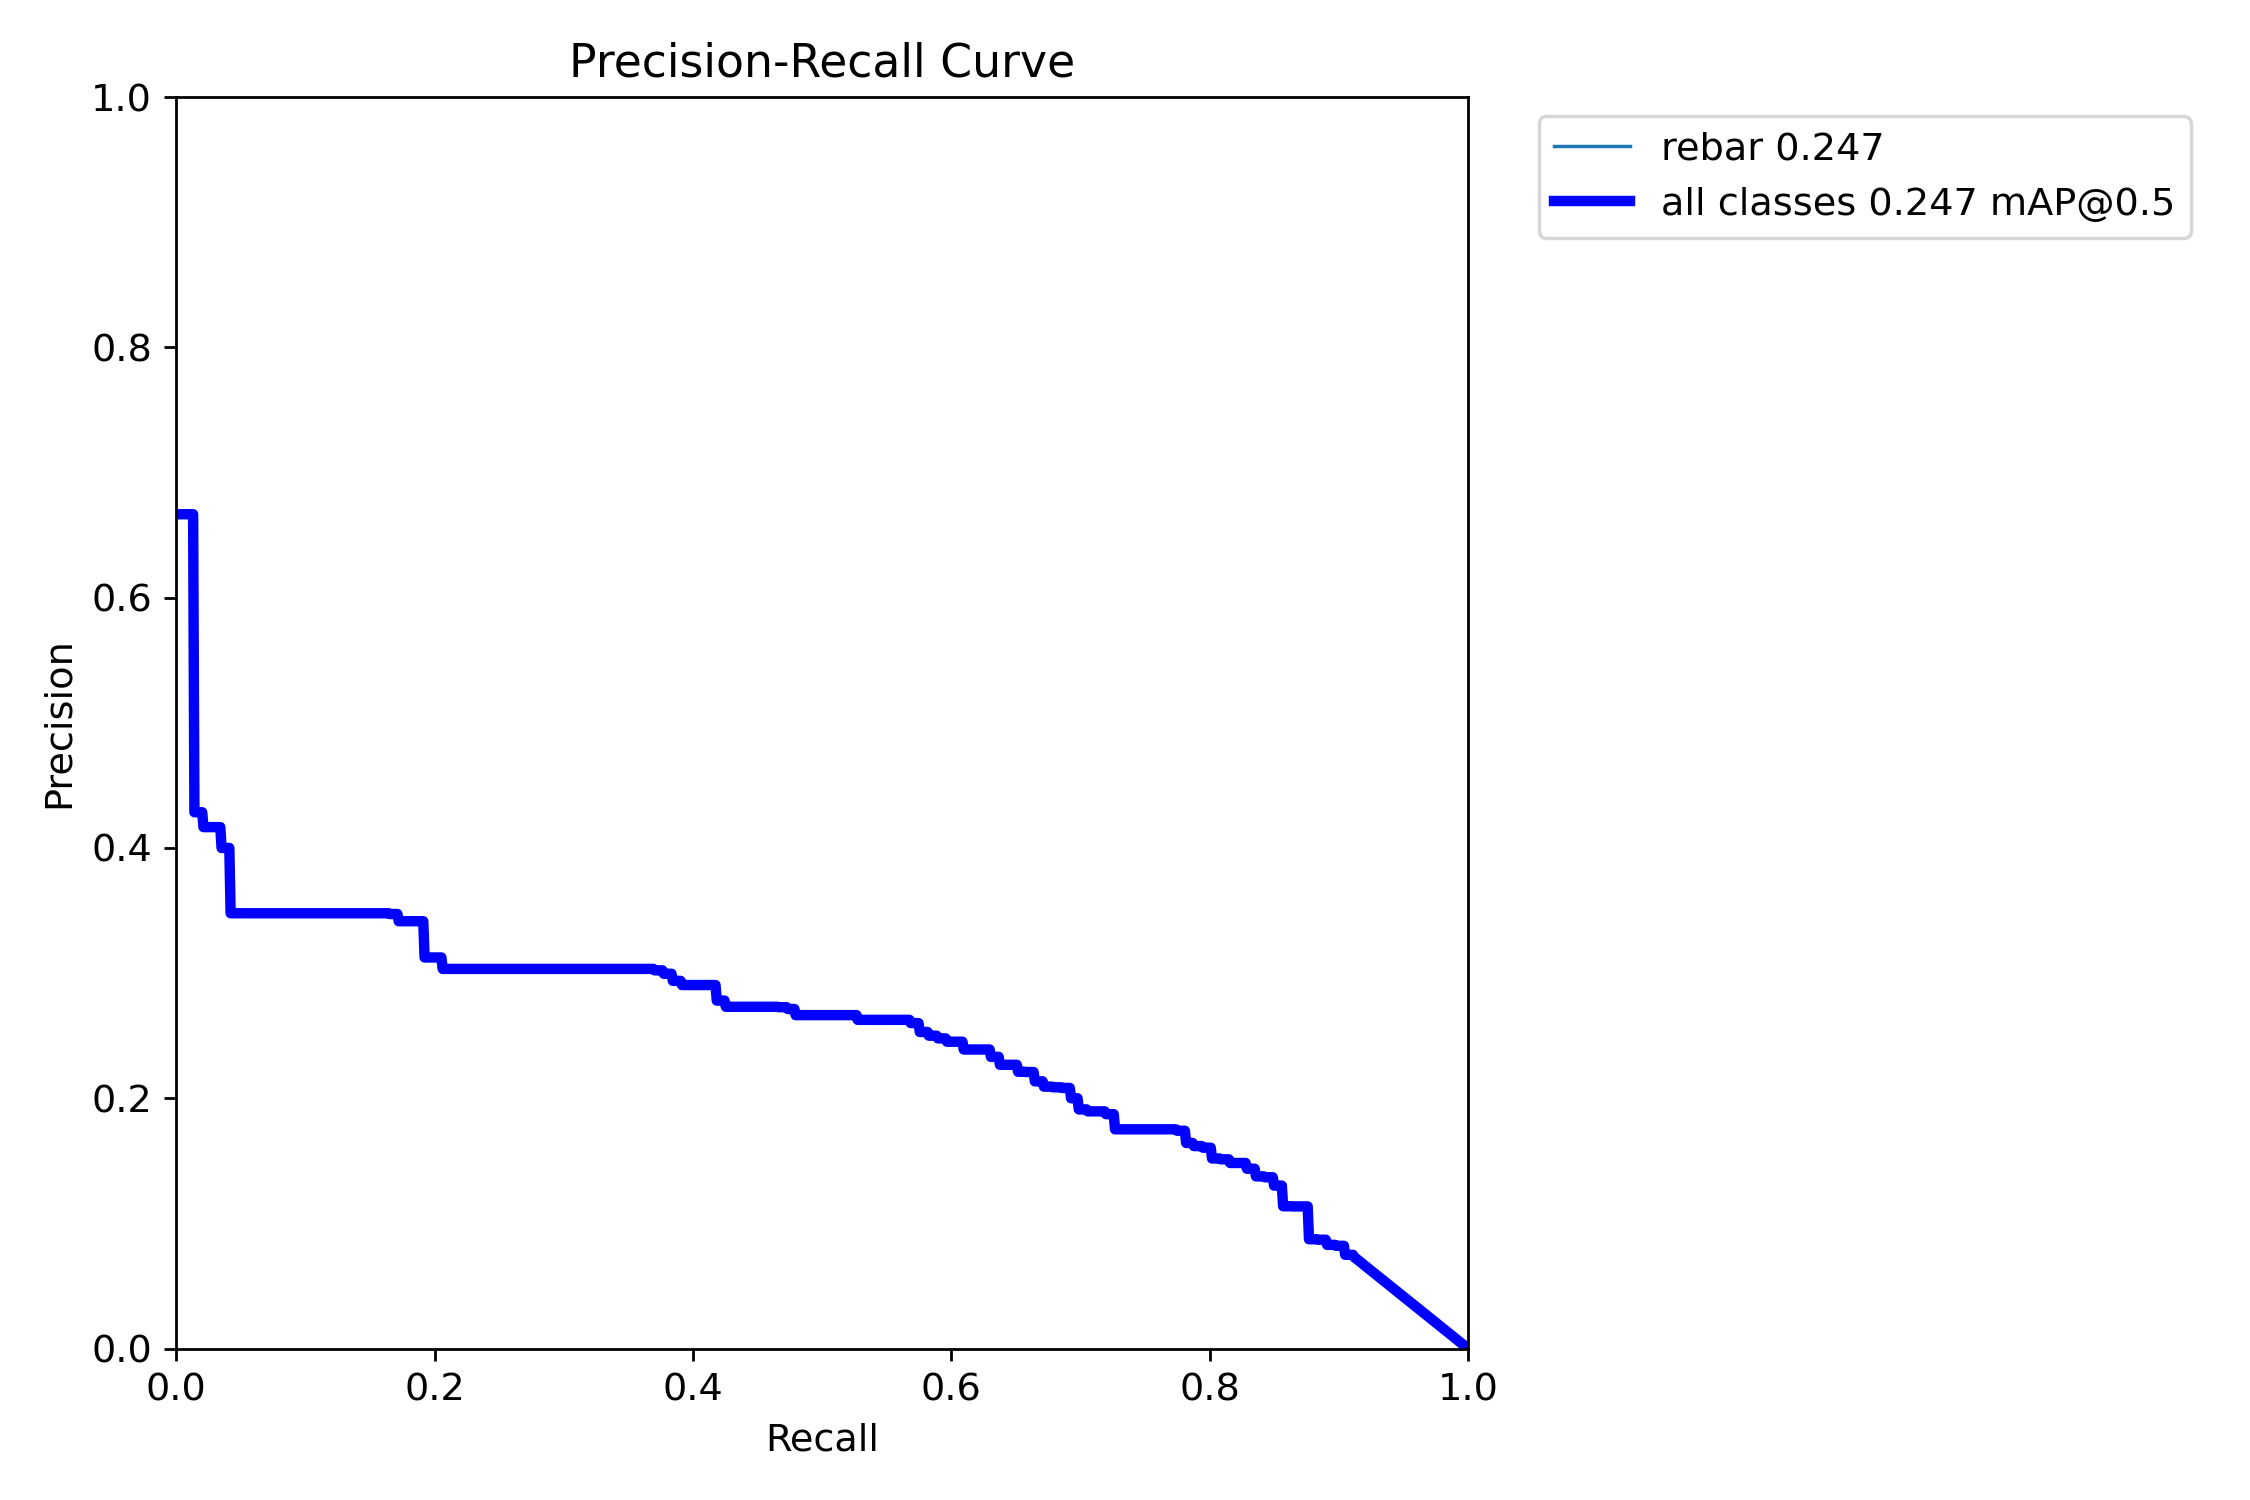
\includegraphics[width=\linewidth]{img/gssi_pr_curve.png}
      \captionof{figure}{GSSI PR curve}
      \label{fig:gssi-pr}
    \end{minipage}\hfill
    \begin{minipage}[t]{0.48\linewidth}
      \centering
      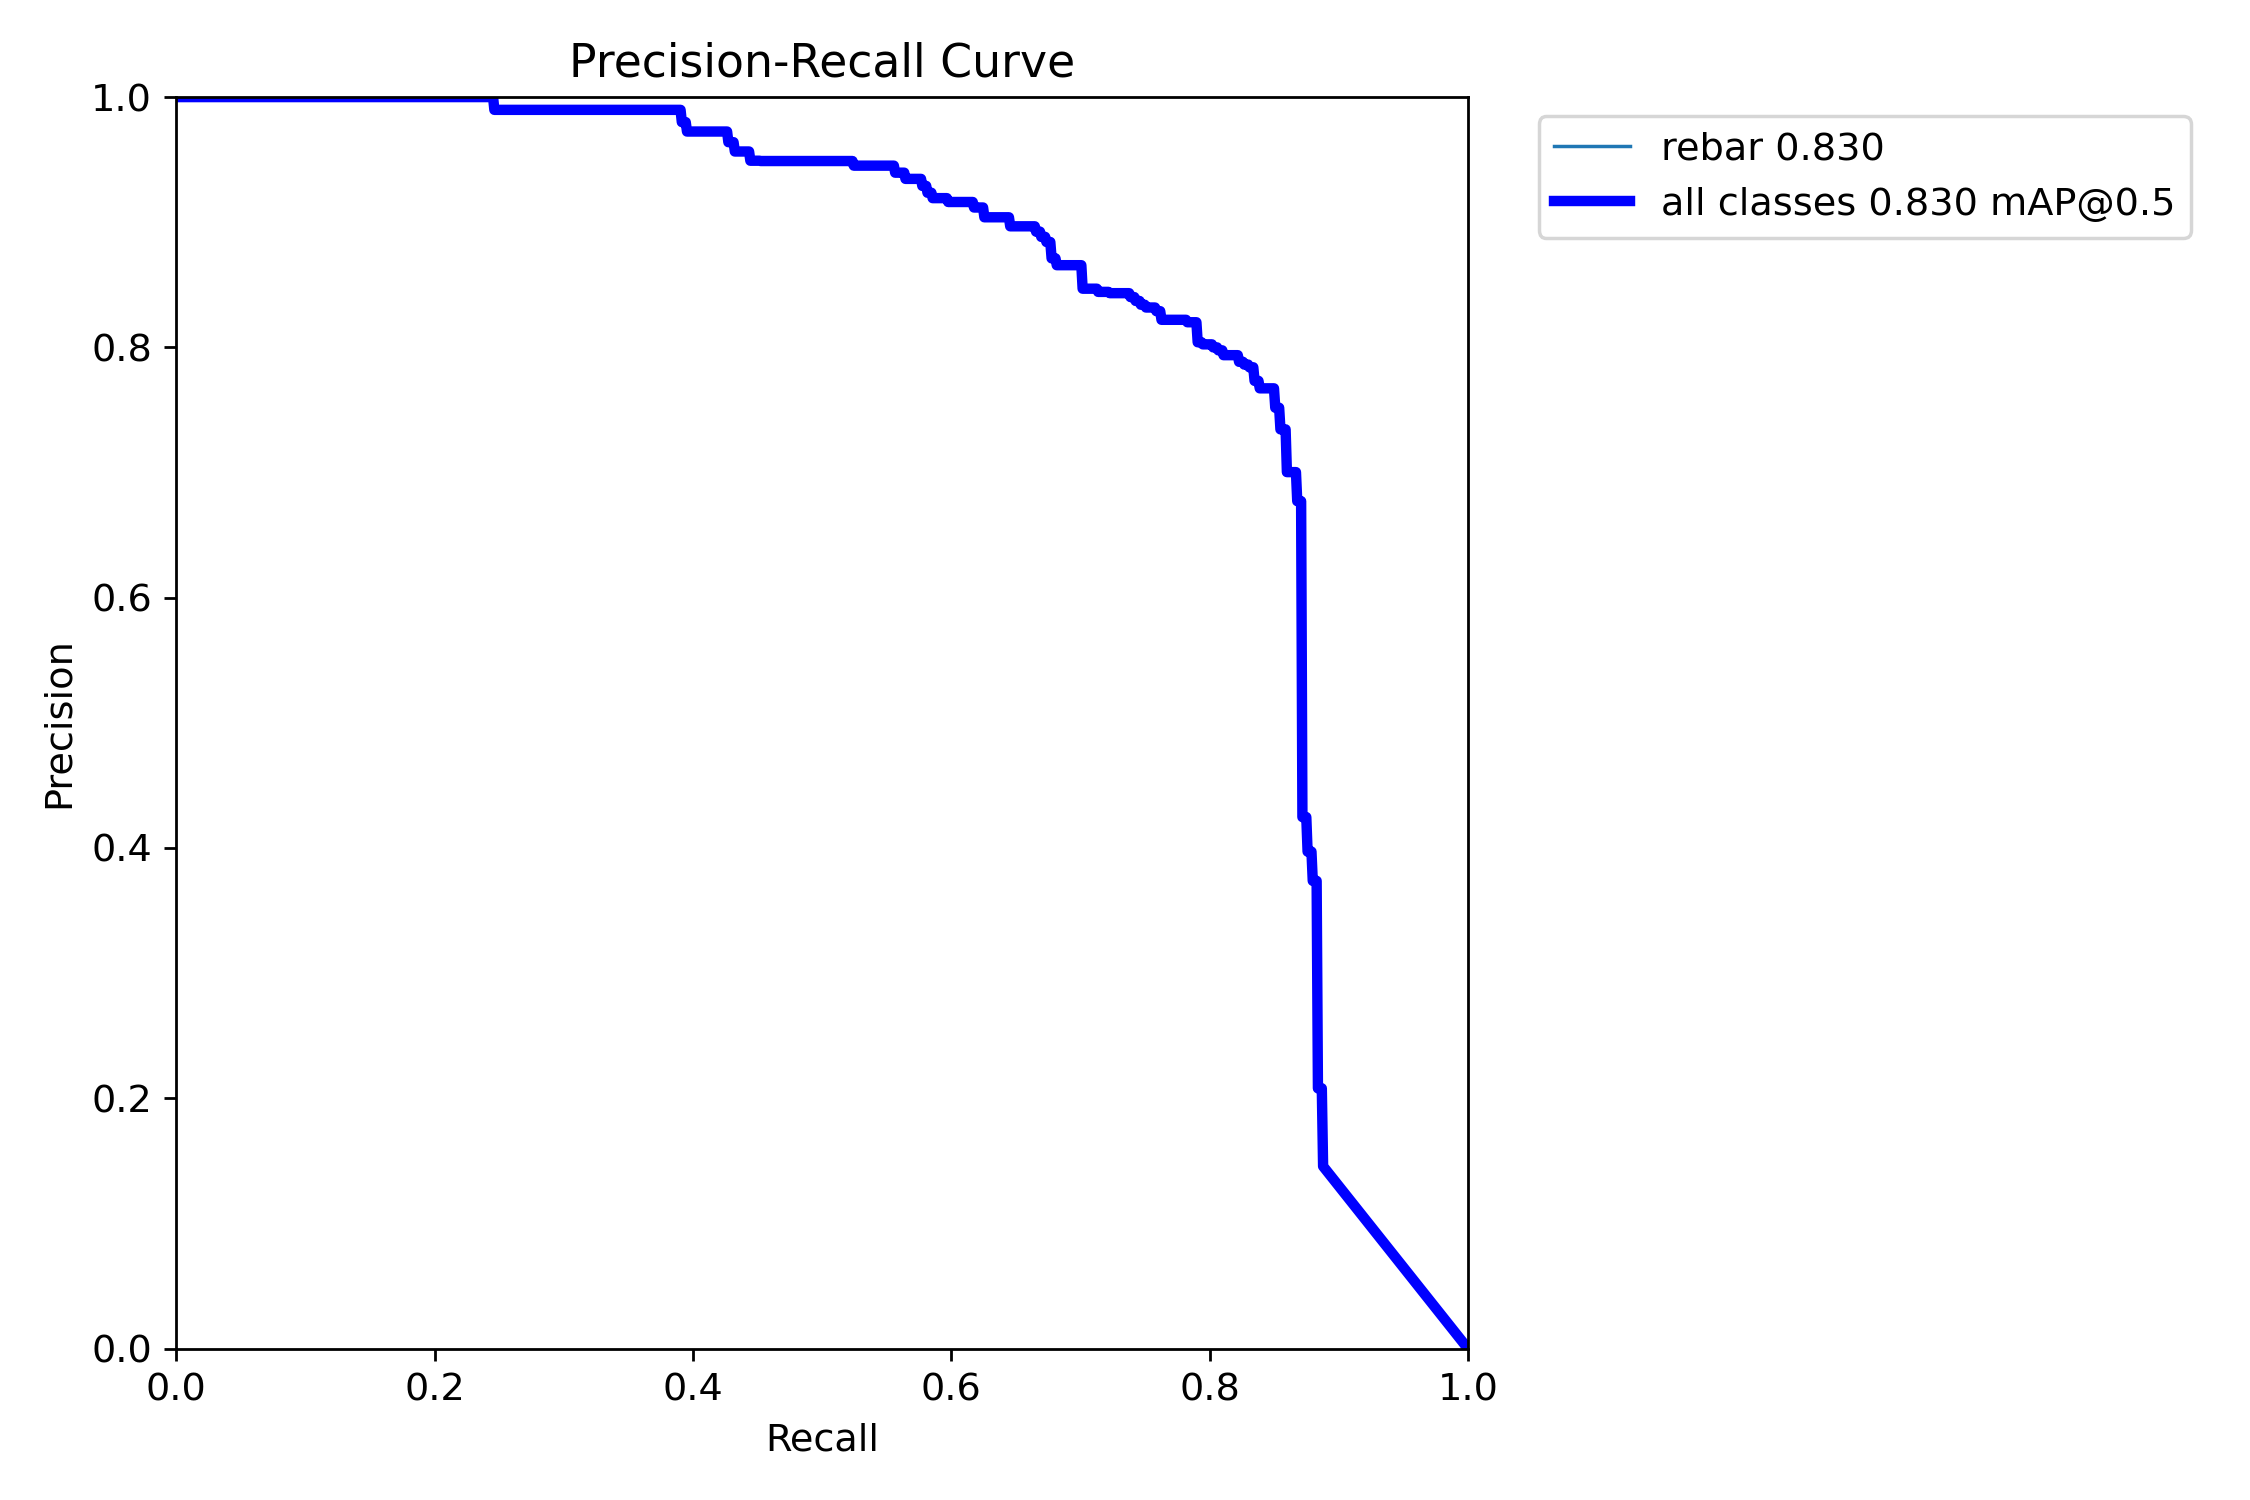
\includegraphics[width=\linewidth]{img/gp8000_pr_curve.png}
      \captionof{figure}{GP8000 PR curve}
      \label{fig:gp8000-pr}
    \end{minipage}

  \end{block}

\end{column}

\separatorcolumn

\begin{column}{\colwidth}

  \begin{block}{Results and Findings}
    \header{Key Results}[0pt]

    \vspace{0.5cm}

    GP8000 YOLOv8n achieves \textbf{mAP@0.5 = 0.830} (P = 0.871, R = 0.857) — production-grade rebar detection on bridge-deck data. GSSI YOLOv8n achieves mAP@0.5 = 0.247 on noisier B-scans; including field data from Georgia DOT will close this gap. Both models exhibit \textbf{near-zero false-positive rates}, confirming that the model learns true hyperbolic echo signatures rather than texture artifacts.

    \header{Key Words}[0pt]

    \emph{ground-penetrating radar, YOLOv8, rebar detection, bridge inspection, deep learning}

    \vspace{0.5cm}

    \begin{figure}[H]
      \centering
      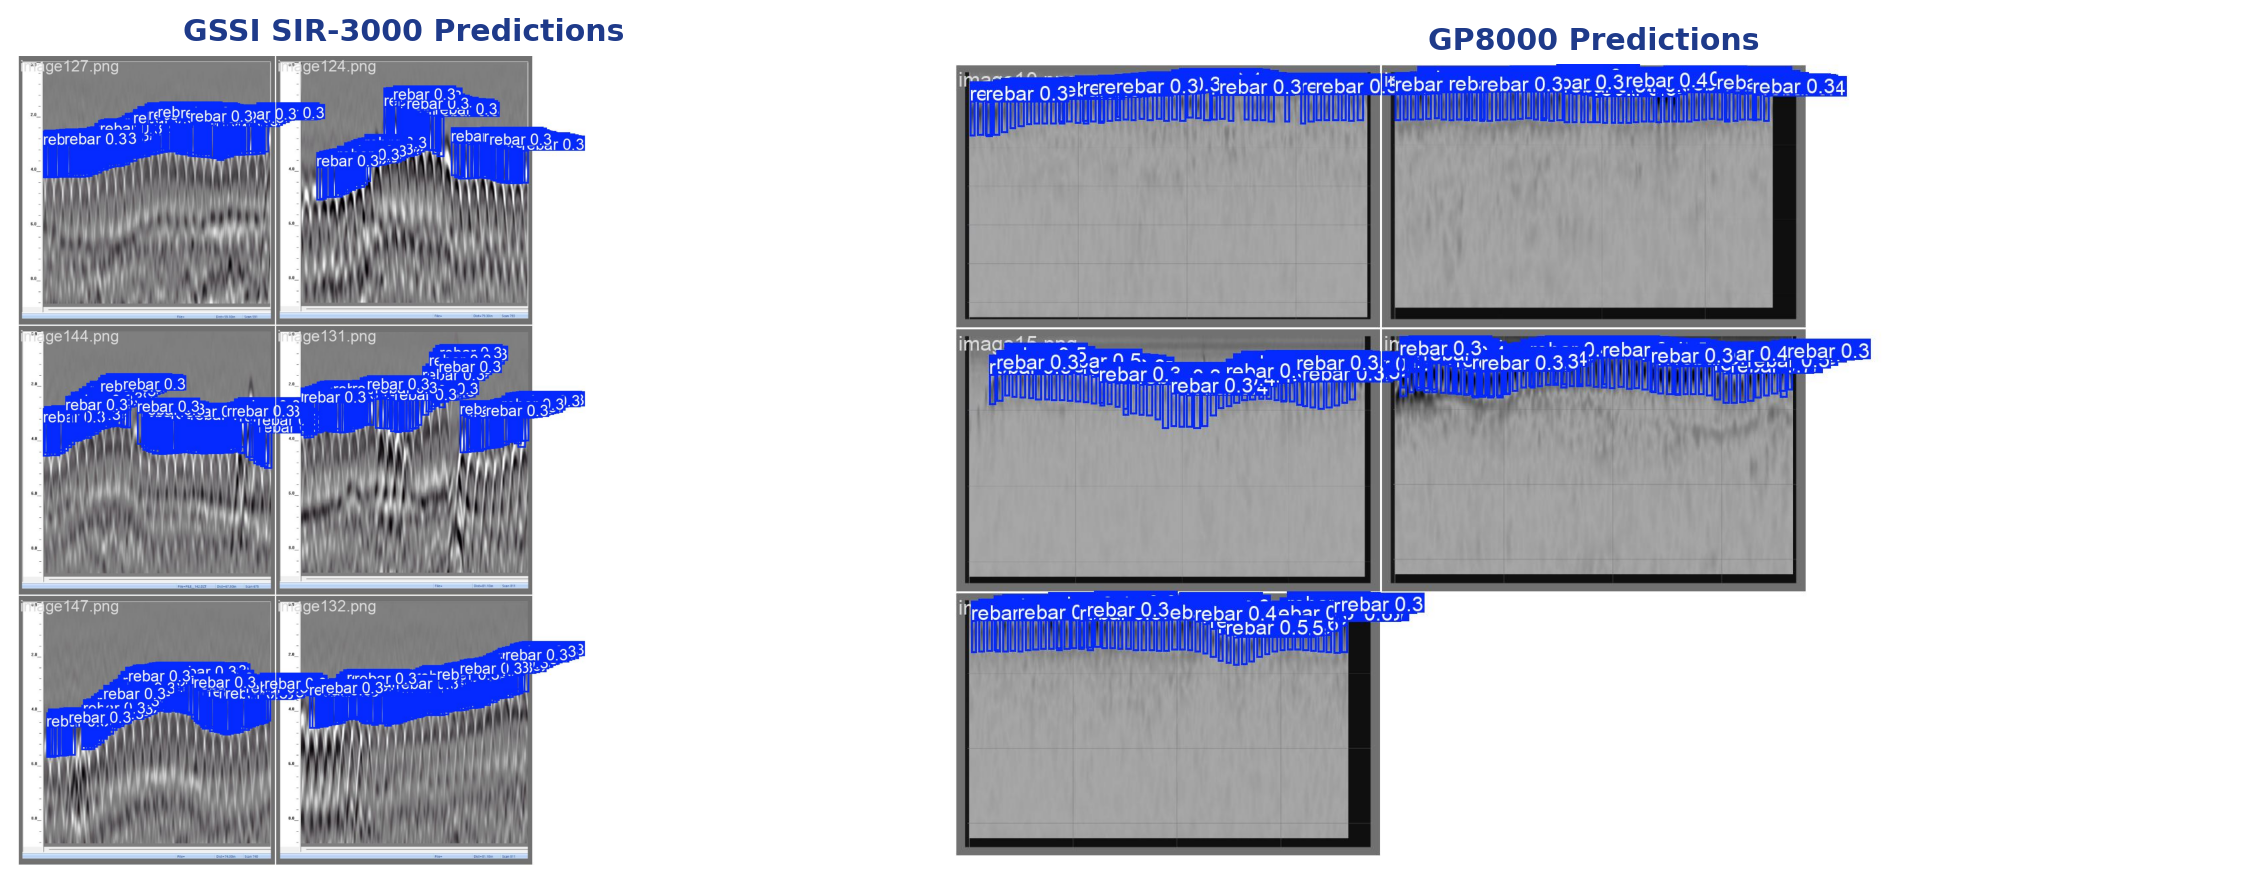
\includegraphics[width=0.95\linewidth]{img/detections_combined.png}
      \caption{Validation predictions: GSSI SIR-3000 (left) and GP8000 (right). Blue boxes = detected rebars.}
      \label{fig:detections}
    \end{figure}

  \end{block}

  \begin{block}{Discussion}
    \header{Interpretation of Results}[0pt]

    \vspace{0.5cm}

    The GP8000 mAP@0.5 $>$ 0.83 validates \textbf{hardware-specific fine-tuning}; cross-hardware unified models perform significantly worse. ConcreteNet GUI is \textbf{field-deployable}: one-click inference, bounding-box editing, PNG export — no Python environment needed. Near-zero background FP rate confirms the model learns true hyperbolic echo signatures, not texture artifacts.

    \header{Implications}[0pt]

    \vspace{0.5cm}

    Bridge inspection costs billions annually. Automated GPR reduces time and variability, enabling earlier corrosion detection. Collaboration with the \textbf{Georgia DOT} will expand the dataset to real bridge-deck scans and add multi-class defect labels (delamination, honeycombing, voids).

    \begin{minipage}[t]{\linewidth}
      \centering
      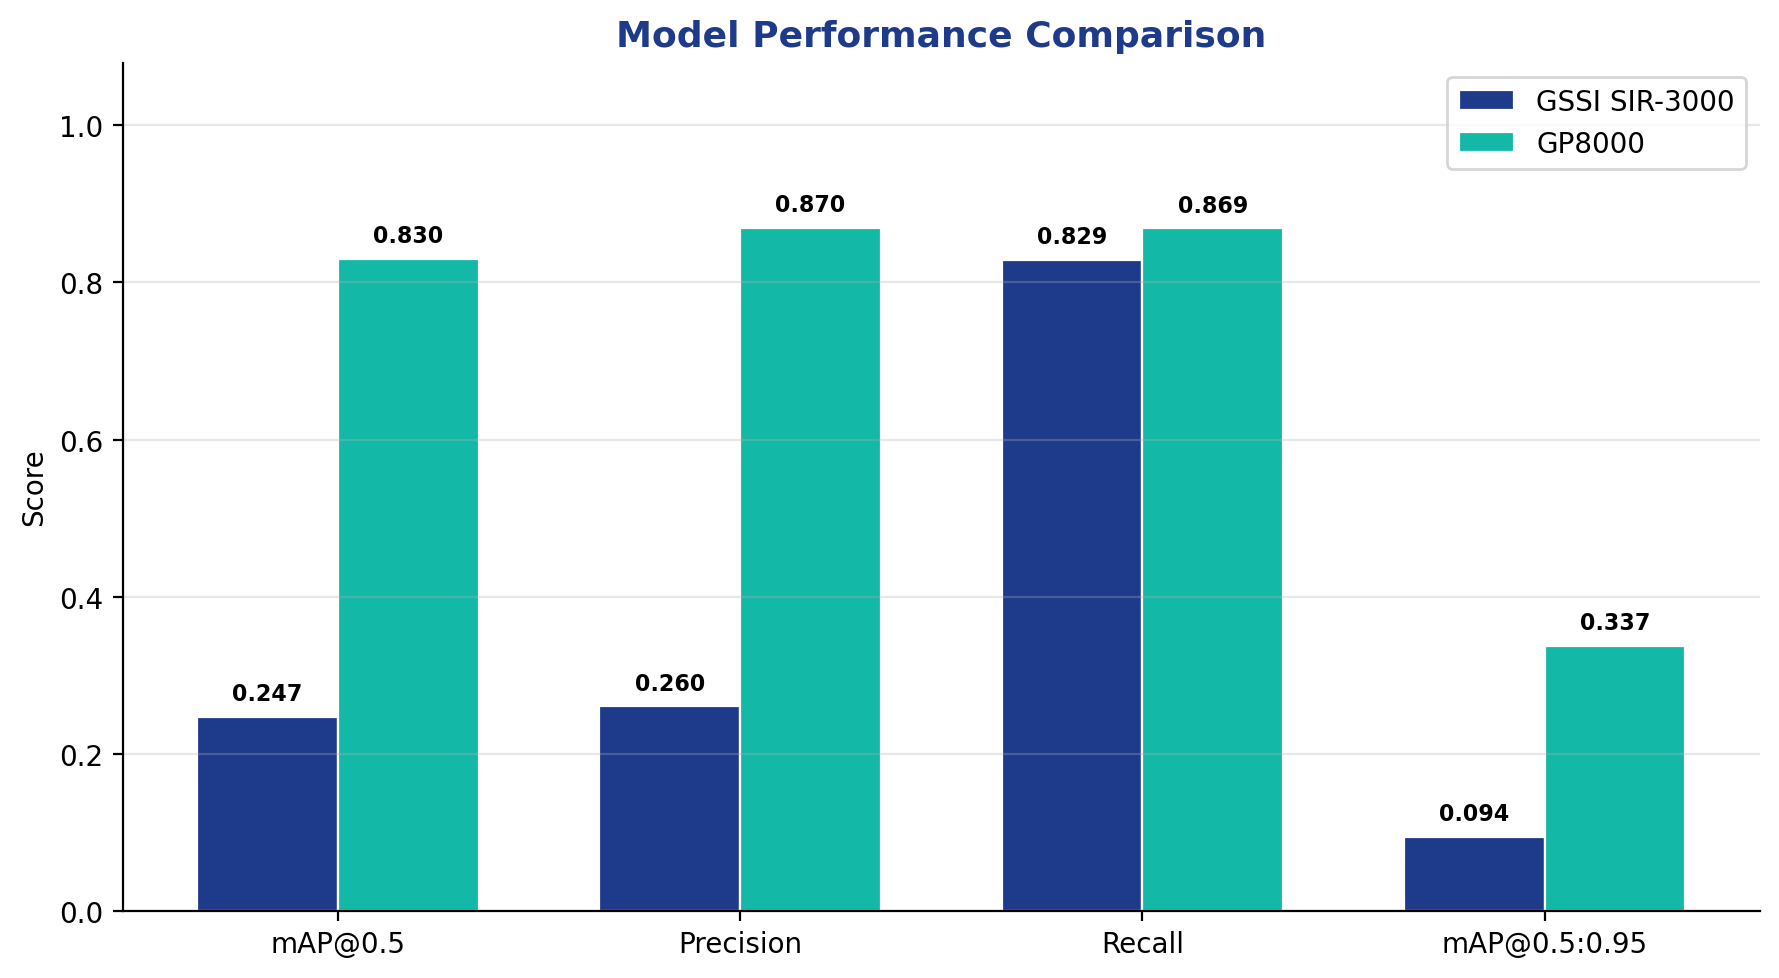
\includegraphics[width=0.9\linewidth, height=0.4\linewidth]{img/perf_bar.png}
      \captionof{figure}{mAP@0.5 comparison: GP8000 vs.\ GSSI SIR-3000}
      \label{fig:perf}
    \end{minipage}

    \vspace{0.5cm}

    More Georgia DOT B-scans and multi-class annotation will further boost GSSI performance and enable defect severity scoring.

    \header{Future Work}[0pt]

    \vspace{0.5cm}

    \begin{itemize}
      \item \textbf{RT-DETR / YOLOv11:} Transformer detectors for context modeling.
      \item \textbf{LSTM:} Sequential modeling across B-scan frames.
      \item \textbf{Public Dataset:} Benchmarked vs.\ RetinaNet, Faster-RCNN, C-MIL.
    \end{itemize}

  \end{block}

  \begin{block}{References / Acknowledgments}

    \begin{hangparas}{.25in}{1}
      Jocher, G., Chaurasia, A., \& Qiu, J. (2023). \textit{Ultralytics YOLO} v8.0.0. github.com/ultralytics/ultralytics
    \end{hangparas}

    \begin{hangparas}{.25in}{1}
      Dinh, K., Gucunski, N., \& Duong, T.H. (2021). Migration-based automated rebar detection from GPR. \textit{NDT \& E International}, 119, 102416.
    \end{hangparas}

    \begin{hangparas}{.25in}{1}
      Giannakis, I.\ \etal (2019). ML for rebar diameter from GPR. \textit{IEEE Geosci. Remote Sens. Lett.}, 18(3), 461--465.
    \end{hangparas}

    \begin{hangparas}{.25in}{1}
      Solla, M., Lorenzo, H., \& Rial, F.I. (2012). GPR assessment with GSSI SIR-3000. \textit{Constr. \& Build. Mat.}, 26(1), 458--465.
    \end{hangparas}

    \vspace{0.5cm}
    \small\textit{Supported by the Allen E.\ Paulson College of Engineering \& Computing and Georgia DOT. GPR data collected from the Georgia Southern Engineering Research Building.}

  \end{block}
\end{column}

\margincolumn
\end{columns}

\begin{tikzpicture}[remember picture, overlay]
  \node[anchor=north east] at ($(current page.north east) + (-4cm, -2.05cm)$) {
      \textbf{\fontsize{100}{0pt}\selectfont \#}
  };
\end{tikzpicture}

\begin{tikzpicture}[remember picture, overlay]
  \node[anchor=north west] at ($(current page.north west) + (0.5in, -7.0cm)$) {
      
\includegraphics[width=0.16\linewidth, height=4.25cm]{img/Georgia_Southern_University_Logo.png}
  };
\end{tikzpicture}

\begin{tikzpicture}[remember picture, overlay]
  % LANDTIE logo — adjust the Y offset here independently
  \node[anchor=south] at ($(current page.south) + (32cm, 107.5cm)$) {
      
\includegraphics[height=8cm]{img/LANDTIE.jpg}
  };
  % Footer text — adjust the Y offset here independently
  \node[anchor=south] at ($(current page.south) + (0, 1.0cm)$) {
      \parbox{60cm}{\centering
      \large\textbf{Allen E.\ Paulson College of Engineering and Computing Student Research Symposium}\\[0.2cm]
      Georgia Southern University \quad\textbullet\quad April 24, 2026}
  };
\end{tikzpicture}


\end{frame}
\end{document}
